%%%%%%%%%%%%%%%%%%%%%%%%%%%%%%%%%%%%%%%%%%%%%%%%%%%%%%%%%%%%%%%%%%%%%%%%%%%%%%%%%%
\begin{frame}[fragile]\frametitle{}
\begin{center}
{\Large Introduction to Machine Learning}
\end{center}
\end{frame}

%%%%%%%%%%%%%%%%%%%%%%%%%%%%%%%%%%%%%%%%%%%%%%%%%%%%%%%%%%%
\begin{frame}[fragile]\frametitle{How do we learn?}
\begin{itemize}
	\item What do we do when we have to prepare for an examination? 
	\item Study. Learn. Imbibe. Take notes. Practice mock papers.
	\item  Thus,  prepare for the unseen test.
	% \item Machine Learning does the same.
\end{itemize}
\end{frame}

%%%%%%%%%%%%%%%%%%%%%%%%%%%%%%%%%%%%%%%%%%%%%%%%%%%%%%%%%%%
\begin{frame}[fragile]\frametitle{What is Learning?}
\begin{center}
{\em ``Learning is any process by which a system improves performance from experience.'' \\}
- Herbert Simon, Turing Award 1975, Nobel in Economics 1978.
\end{center}

% \begin{center}
% {\em ``Machine Learning is concerned with computer programs that automatically improve their performance through experience.''}\\
% %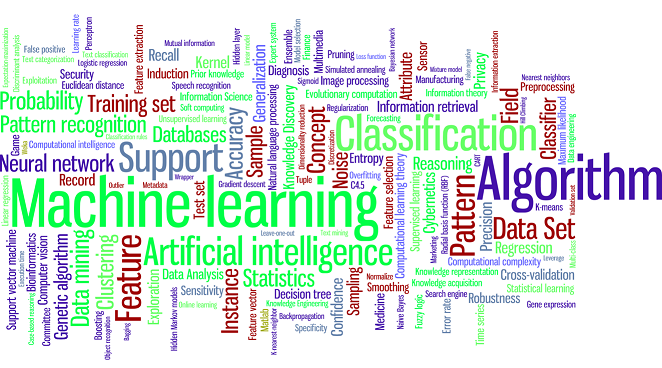
\includegraphics[width=0.9\linewidth,keepaspectratio]{mlcloud}
% \end{center}
\end{frame}



%%%%%%%%%%%%%%%%%%%%%%%%%%%%%%%%%%%%%%%%%%%%%%%%%%%%%%%%%%
\begin{frame}[fragile]\frametitle{What is Machine Learning?}
Machine learning is a type of artificial intelligence (AI) which:
\begin{itemize}
\item Learns function without being explicitly programmed. 
\item Can grow and change when exposed to new data. 
\end{itemize}
\end{frame}

%%%%%%%%%%%%%%%%%%%%%%%%%%%%%%%%%%%%%%%%%%%%%%%%%%%%%%%%%%
\begin{frame}[fragile]\frametitle{Quick Definition}
{\it Machine learning is a field of study that gives computers the ability to learn, without being explicitly programmed.}

- Arthur Samuel, 1959

So, rather than coding each step explicitly, you give computers just some examples, and it figures out the steps.
\end{frame}

%%%%%%%%%%%%%%%%%%%%%%%%%%%%%%%%%%%%%%%%%%%%%%%%%%%%%%%%%%%
\begin{frame}[fragile]\frametitle{Another Definition of Machine Learning}
Machine learning is manifestation of statistical learning: implemented through software.
\end{frame}


%%%%%%%%%%%%%%%%%%%%%%%%%%%%%%%%%%%%%%%%%%%%%%%%%%%%%%%%%%
\begin{frame}[fragile]\frametitle{WellPosed Definition}



{\it A computer program is said to learn from experience E with respect to some class of tasks T and some performance measure P, if its performance at tasks in T, as measured by P, improves with experience E.}

- T. Mitchell's book Machine Learning (1997)

In the various problem settings T, P, and E can refer to completely different things. 
\end{frame}

%%%%%%%%%%%%%%%%%%%%%%%%%%%%%%%%%%%%%%%%%%%%%%%%%%%%%%%%%%
\begin{frame}[fragile]\frametitle{Intuition}
\begin{itemize}
\item For any process (Machine ie Artificial or Biological), need to define a task, say Spam Detection. Machine can also do it and humans can also detect it.
\item Experience means multiple observations, runs, practices. So in our examples, its more Spam/Non-Spam examples.
\item Performance defined is How many we got right ie Accuracy.
\item Now if Task of Spam detection improves Accuracy if we look at more samples, then this is Machine Learning.
\item Its also called Inductive Learning (``Learning by Experience''). Based on evidence (not Facts), so its suggestive.
\item Another type is deductive (inferences based on facts/rules. So, more deterministic. Eg I went to Movie today. Today is Saturday. Inference: I went to movie on Saturday.)
\end{itemize}
\end{frame}

%%%%%%%%%%%%%%%%%%%%%%%%%%%%%%%%%%%%%%%%%%%%%%%%%%%%%%%%%%
\begin{frame}[fragile]\frametitle{Intuition}
\begin{itemize}
\item Mitchell's definition, though looks OK for Machine Learning, its not very rigorous.
\item Contrary example: Say your task is Bike driving, experiences is more miles you drive, performance is smoothness of drive (vibrations).
\item As you put more miles, due to smoothening, performance improves (vibrations go down), is it Learning? 
\item No!!!
\item But for Machine Learning domain, it looks fine.
\end{itemize}
\end{frame}

%%%%%%%%%%%%%%%%%%%%%%%%%%%%%%%%%%%%%%%%%%%%%%%%%%%%%%%%%%
\begin{frame}[fragile]\frametitle{Tasks}
Tasks T in machine learning
\begin{itemize}
\item Classification of an instance to one of the categories based on its features;
\item Regression – prediction of a numerical target feature based on other features of an instance;
\item Clustering – identifying partitions of instances based on the features of these instances so that the members within the groups are more similar to each other than those in the other groups;
\item etc
\end{itemize}
\end{frame}


%%%%%%%%%%%%%%%%%%%%%%%%%%%%%%%%%%%%%%%%%%%%%%%%%%%%%%%%%%
\begin{frame}[fragile]\frametitle{Experience}
\begin{itemize}
\item Experience E refers to data (we can't go anywhere without it).
\item For example, to predict loan defaults based on the data accumulated about our clients. 
\item Here, the experience E is the available training data: a set of instances (clients), a collection of features (such as age, salary, type of loan, past loan defaults, etc.) for each, 
\item And a target variable (whether they defaulted on the loan) is (1 or 0), 
\item This is a (binary) classification problem. 
\end{itemize}
\end{frame}

%%%%%%%%%%%%%%%%%%%%%%%%%%%%%%%%%%%%%%%%%%%%%%%%%%%%%%%%%%
\begin{frame}[fragile]\frametitle{Performance}
\begin{itemize}
\item Metric of the algorithm's performance evaluation P
\item Such metrics differ for various problems and algorithms
\item A simple metric for classification algorithms, the proportion of correct answers – accuracy – on the test set.
\end{itemize}
\end{frame}


%%%%%%%%%%%%%%%%%%%%%%%%%%%%%%%%%%%%%%%%%%%%%%%%%%%%%%%%%%%
\begin{frame}[fragile]\frametitle{So, What is Machine Learning?}
\begin{itemize}
\item Ability of computers to ``learn'' from ``data''
\item Learn: Discover patterns, underlying structure  
\item Data: Comes from sensors, transactions, etc.
\end{itemize}
\end{frame}


%%%%%%%%%%%%%%%%%%%%%%%%%%%%%%%%%%%%%%%%%%%%%%%%%%%%%%%%%%%
\begin{frame}[fragile]\frametitle{Goal of Statistical learning}
Dependent variables need to predicted or estimated in terms of independent variables.

	\begin{itemize}
	\item Data in control: independent variables.
	\item Data not in control: dependent variables.
	\end{itemize}
\end{frame}

%%%%%%%%%%%%%%%%%%%%%%%%%%%%%%%%%%%%%%%%%%%%%%%%%%%%%%%%%%%
\begin{frame}[fragile]\frametitle{Example}
 Goal: to measure sales based on the advertising budget allocated for TV, Radio, and Print.
\begin{itemize}
\item Can control: budgets of TV, Radio, and Print. 
\item Cannot control: how they will impact the sales. 
\item Express dependent (sales) as function of independent (advertising budget). 
\item Want to uncover this hidden relationship.
\item Statistical learning reveals hidden data relationships. 
\item Relationships between dependent and independent data.
\end{itemize}
\end{frame}

%%%%%%%%%%%%%%%%%%%%%%%%%%%%%%%%%%%%%%%%%%%%%%%%%%%%%%%%%%%
\begin{frame}[fragile]\frametitle{Mathematical Definition of Machine Learning}
Machine Learning comes up with a Model given inputs and targets.

\begin{itemize}
\item Input data is available. 
\item Input data is transformed to get output.
\item Output: something that needs to be predicted or estimated.
\item Transformation engine is called Model or function.
\end{itemize}
\end{frame}

%%%%%%%%%%%%%%%%%%%%%%%%%%%%%%%%%%%%%%%%%%%%%%%%%%%%%%%%%%%
\begin{frame}[fragile]\frametitle{Model entities}
For $income = c + \beta_0 \times education + \beta_1 \times experience$
\begin{itemize}
\item Inputs: Education and experience, also called as features or attributes or dimensions or variables.
\item Mathematical entities added to input data, are Parameters.. $\beta_0$ and $\beta_1$ are parameters
\item Income is target, also called as outcome or class.
\end{itemize}
\end{frame}

%%%%%%%%%%%%%%%%%%%%%%%%%%%%%%%%%%%%%%%%%%%%%%%%%%%%%%%%%%%
\begin{frame}[fragile]\frametitle{Traditional vs. Machine Learning?}
\begin{center}
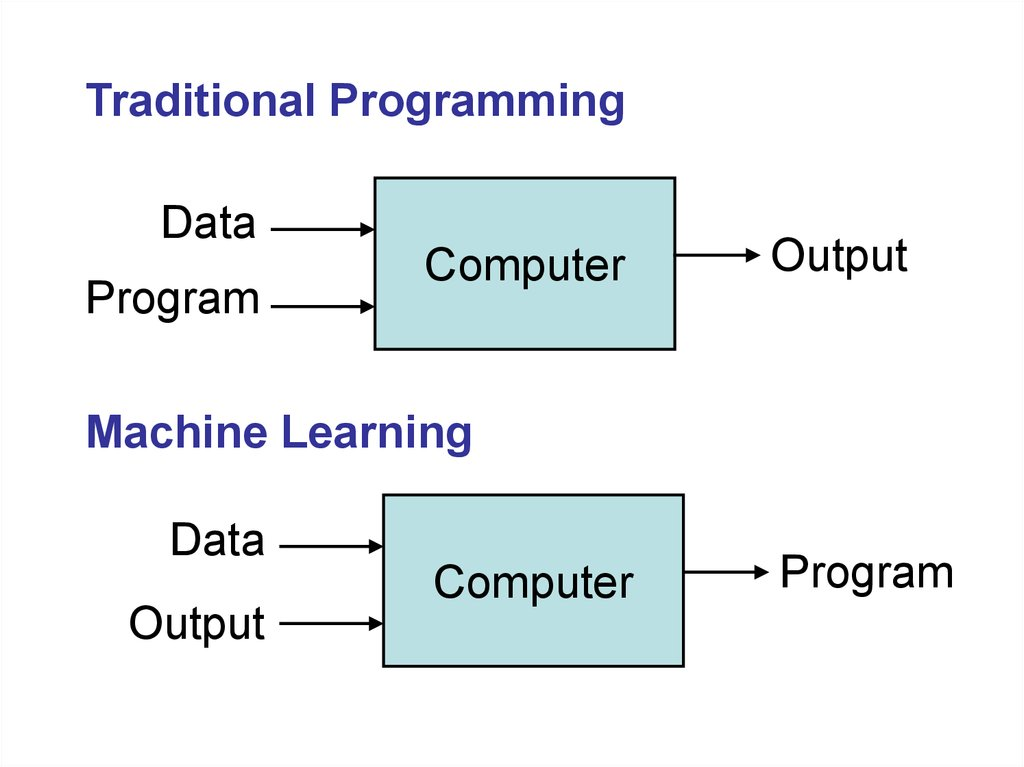
\includegraphics[width=0.8\linewidth,keepaspectratio]{tradml}
\end{center}
\end{frame}

%%%%%%%%%%%%%%%%%%%%%%%%%%%%%%%%%%%%%%%%%%%%%%%%%%%%%%%%%%%
\begin{frame}[fragile]\frametitle{Why Machine Learning?}
\begin{itemize}
\item Problems with High Dimensionality
\item Hard/Expensive to program manually
\item Techniques to model `ANY' function given `ENOUGH' data.
\item Job \$\$\$
\end{itemize}
%\begin{center}
%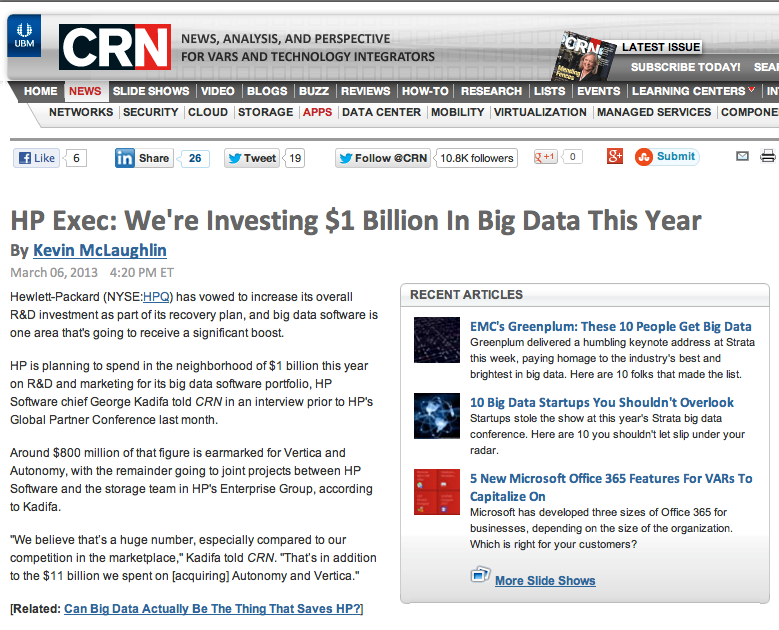
\includegraphics[width=0.45\linewidth,keepaspectratio]{hp}
%\end{center}
\end{frame}

%%%%%%%%%%%%%%%%%%%%%%%%%%%%%%%%%%%%%%%%%%%%%%%%%%%%%%%%%%
\begin{frame}[fragile]\frametitle{Machine Learning Process}
\begin{center}
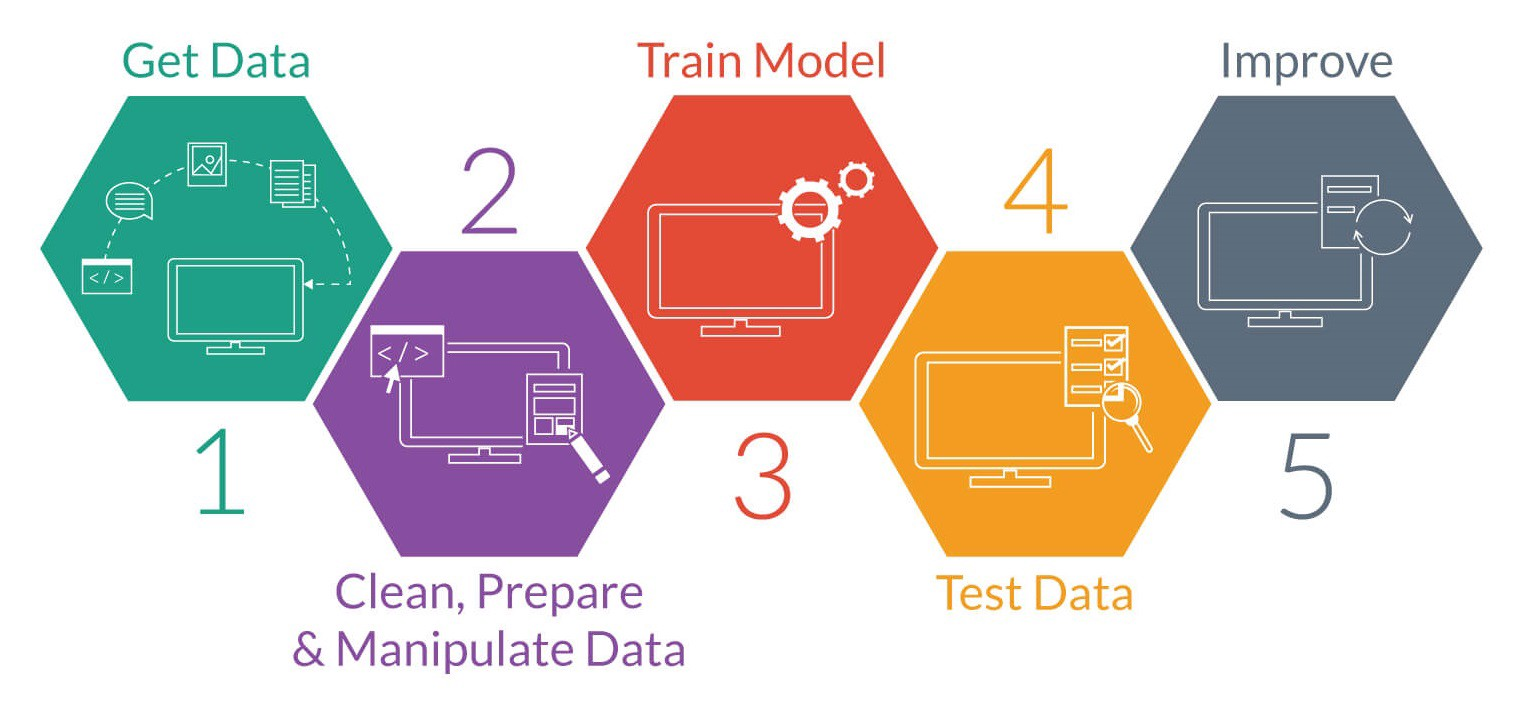
\includegraphics[width=\linewidth,keepaspectratio]{mlteq2}
\end{center}
\tiny{(Reference: The Role of Big Data in Strengthening Machine Learning Projects - Techno FAQ)}
\end{frame}


%%%%%%%%%%%%%%%%%%%%%%%%%%%%%%%%%%%%%%%%%%%%%%%%%%%%%%%%%%%
\begin{frame}[fragile]\frametitle{Why now?}
\begin{itemize}
\item Flood of data (Internet, IoT)
\item Increasing computational power
\item Easy/free availability of algorithms 
\item Increasing support from industries
\end{itemize}
\end{frame}

% %%%%%%%%%%%%%%%%%%%%%%%%%%%%%%%%%%%%%%%%%%%%%%%%%%%%%%%%%%%
% \begin{frame}[fragile]\frametitle{Challenges}
% Scalability
	% \begin{itemize}
	% \item Gigabytes, Tera-bytes, Peta-bytes, Hexa-bytes
	% \item Storage capacity, streaming?
	% \item Limits of python libraries
	% \end{itemize}
% \end{frame}

% %%%%%%%%%%%%%%%%%%%%%%%%%%%%%%%%%%%%%%%%%%%%%%%%%%%%%%%%%%%
% \begin{frame}[fragile]\frametitle{Challenges}
% High Dimensionality
	% \begin{itemize}
	% \item Datasets with hundreds or thousands of attributes
	% \item Many variables are collected; few turn out to be useful
	% \end{itemize}
% Heterogeneous and Complex Data
% \end{frame}


% %%%%%%%%%%%%%%%%%%%%%%%%%%%%%%%%%%%%%%%%%%%%%%%%%%%%%%%%%%%
% \begin{frame}[fragile]\frametitle{Data:Oil}
% \begin{center}
% {\em ``Data is the new oil. It's valuable, but if unrefined it cannot be used. It has to be changed into gas, plastic, chemicals, etc. to create a valuable entity that drives profitable activity; so, must data be broken down, analyzed for it to have value. ''}\\
% - Clive Humbly, UK Mathematician, 2006
% \end{center}
% \begin{center}
% 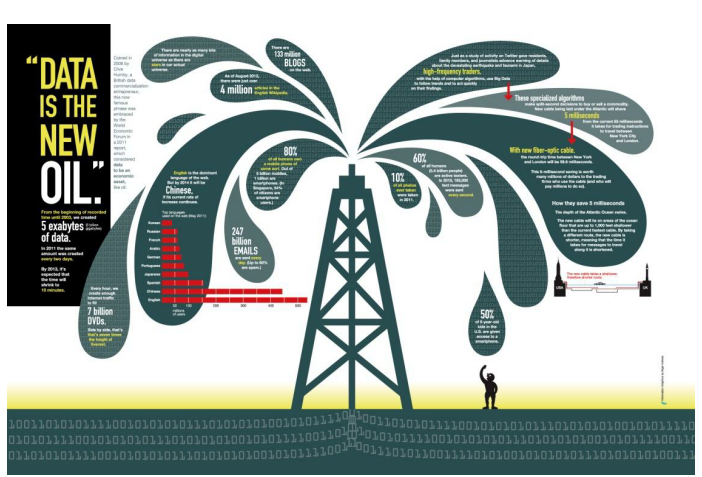
\includegraphics[width=0.5\linewidth,keepaspectratio]{dataoil}
% \end{center}
% {\tiny (Reference: ``Futuretext'' - Ajit Jaokar)}
% \end{frame}
%%%%%%%%%%%%%%%%%%%%%%%%%%%%%%%%%%%%%%%%%%%%%%%%%%%%%%%%%%%
\begin{frame}[fragile]\frametitle{The storm: The Big Data is coming}
\begin{itemize}
\item In 2012, HBR put Data Scientists on the radar
\item ``The Sexiest Job of the 21st Century''.
\item Industry, trying to be data-driven, than manual.
\end{itemize}
%\begin{center}
%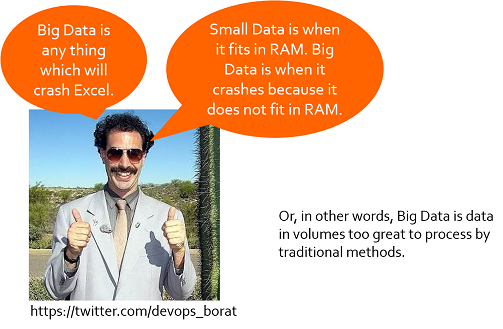
\includegraphics[width=0.7\linewidth,keepaspectratio]{bigdata}
%\end{center}
\end{frame}



%%%%%%%%%%%%%%%%%%%%%%%%%%%%%%%%%%%%%%%%%%%%%%%%%%%
\begin{frame}[fragile] \frametitle{(Big) Data Characteristics}
\begin{center}
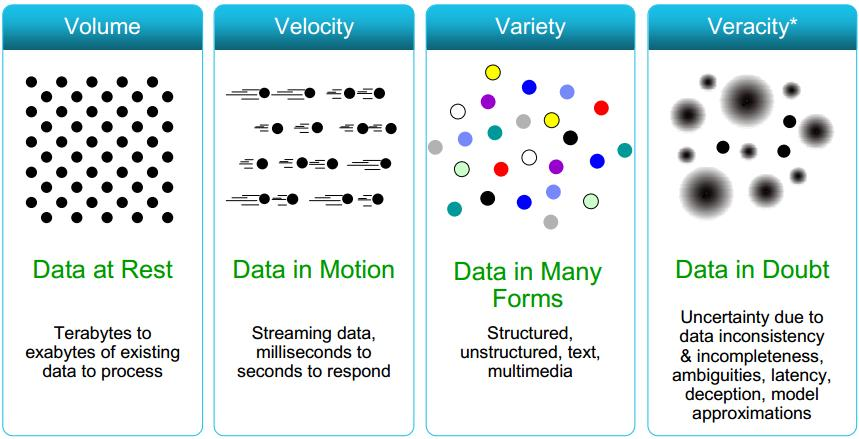
\includegraphics[width=\linewidth,keepaspectratio]{datachar}
\end{center}
{\tiny (Image Credit: http://www.rosebt.com/blog/data-veracity)}
\end{frame}


%%%%%%%%%%%%%%%%%%%%%%%%%%%%%%%%%%%%%%%%%%%%%%%%%%%%%%%%%%%
\begin{frame}[fragile]\frametitle{What's the answer?}
AI-ML-DL
\begin{itemize}
\item Machines showing intelligence of Humans
\item Machine Learning: part of AI
\item Logic is not programmed by hand, 
\item Gets emerged in training with data.
\end{itemize}
\end{frame}

% %%%%%%%%%%%%%%%%%%%%%%%%%%%%%%%%%%%%%%%%%%%%%%%%%%%%%%%%%%%
% \begin{frame}[fragile]\frametitle{Is AI an answer?}
% \begin{center}
% 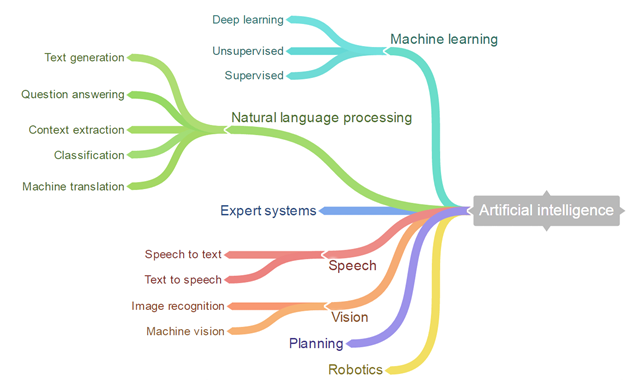
\includegraphics[width=\linewidth,keepaspectratio]{aiml}
% \end{center}
% {\tiny (https://hackernoon.com/jump-start-to-artificial-intelligence-f6eb30d624ec)}
% \end{frame}

%%%%%%%%%%%%%%%%%%%%%%%%%%%%%%%%%%%%%%%%%%%%%%%%%%%%%%%%%%%%%%%%%%%%%%%%%%%%%%%%%%
\begin{frame}[fragile]\frametitle{}
\begin{center}
{\Large A Puzzle}
\end{center}
\end{frame}

%%%%%%%%%%%%%%%%%%%%%%%%%%%%%%%%%%%%%%%%%%%%%%%%%%%%%%%%%%%
\begin{frame}[fragile]\frametitle{How different is Machine Learning?}
Maths Puzzle
\begin{center}
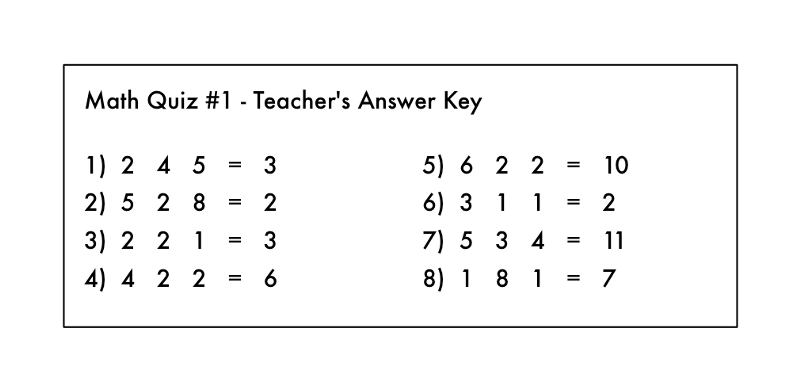
\includegraphics[width=\linewidth,keepaspectratio]{mathspuzz}
\end{center}
\end{frame}

%%%%%%%%%%%%%%%%%%%%%%%%%%%%%%%%%%%%%%%%%%%%%%%%%%%%%%%%%%%
\begin{frame}[fragile]\frametitle{Maths Puzzle}
\begin{itemize}
\item Letting the computer work out that relationship for you. 
\item `Learn' to solve such problems, 
\item `Test' with any other problem of the same type!
\end{itemize}
\end{frame}

%
%%%%%%%%%%%%%%%%%%%%%%%%%%%%%%%%%%%%%%%%%%%%%%%%%%%%%%%%%%%%
%\begin{frame}[fragile]\frametitle{Machine Learning Applications}
%\begin{center}
%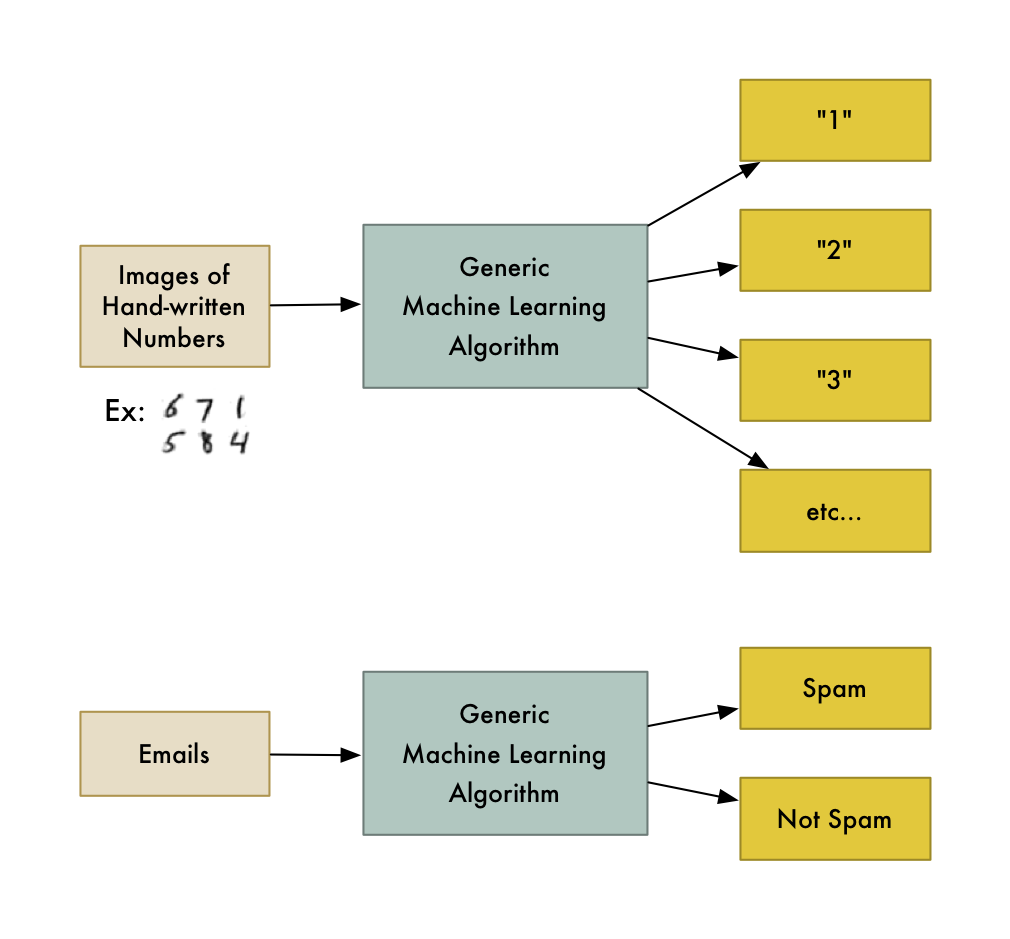
\includegraphics[width=0.6\linewidth,keepaspectratio]{mlapps}
%\end{center}
% Instead of writing code, you feed data to the generic algorithm and it builds its own logic based on the data.
%\end{frame}
%
%
%%%%%%%%%%%%%%%%%%%%%%%%%%%%%%%%%%%%%%%%%%%%%%%%%%%%%%%%%%%%
%\begin{frame}[fragile]\frametitle{Machine Learning Applications}
%\begin{center}
%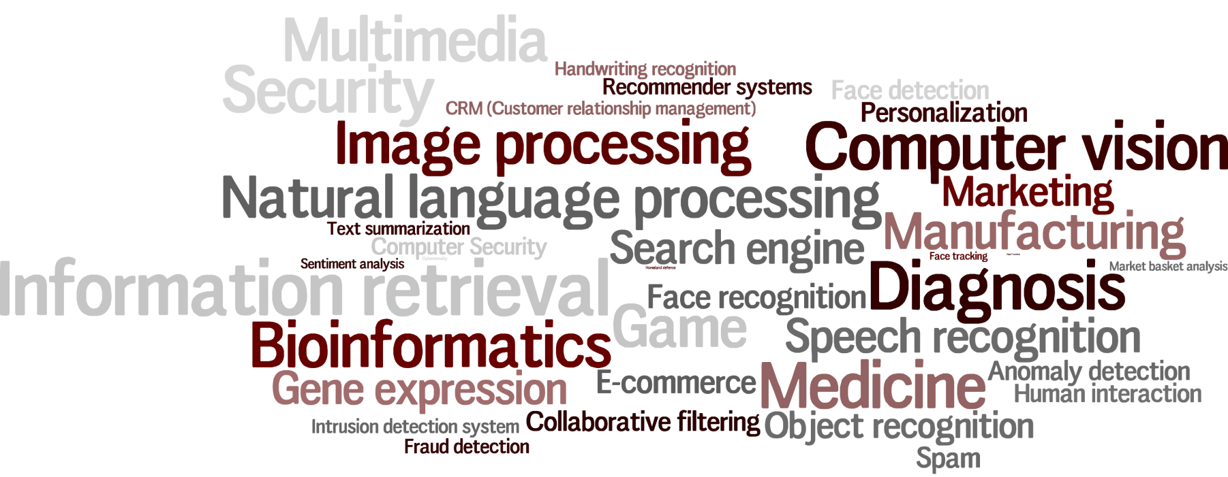
\includegraphics[width=\linewidth,keepaspectratio]{mlapplns}
%\end{center}
%\end{frame}
%
%%%%%%%%%%%%%%%%%%%%%%%%%%%%%%%%%%%%%%%%%%%%%%%%%%%%%%%%%%%%
%\begin{frame}[fragile]\frametitle{Machine Learning, continuation of Data Mining}
%\begin{itemize}
%\item Data Mining/ Business Analytics/Business Intelligence?
%\item Analyze data for decision making
%\item Trying to get insights
%\item Machine Learning: prediction, classification, etc.
%\item Moving from data to insights to future decisions.
%\end{itemize}
%\end{frame}

% %%%%%%%%%%%%%%%%%%%%%%%%%%%%%%%%%%%%%%%%%%%%%%%%%%%%%%%%%%%
% \begin{frame}[fragile]\frametitle{Machine Learning, continuation of Data Mining}
% \begin{center}
% 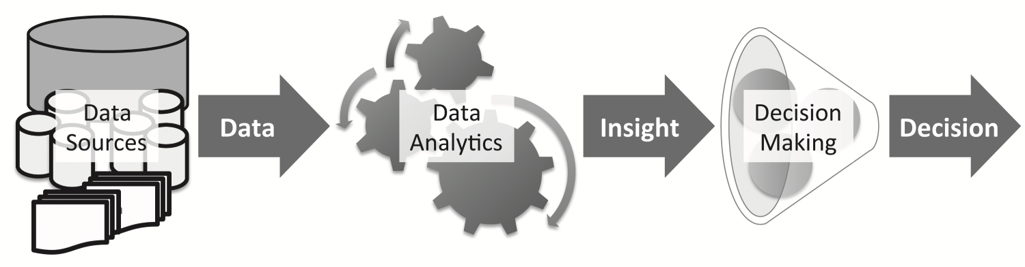
\includegraphics[width=\linewidth,keepaspectratio]{predict}
% \end{center}
% \end{frame}

%%%%%%%%%%%%%%%%%%%%%%%%%%%%%%%%%%%%%%%%%%%%%%%%%%%%%%%%%%%%
%\begin{frame}[fragile]\frametitle{Data Mining/ Machine Learning Process}
%\begin{center}
%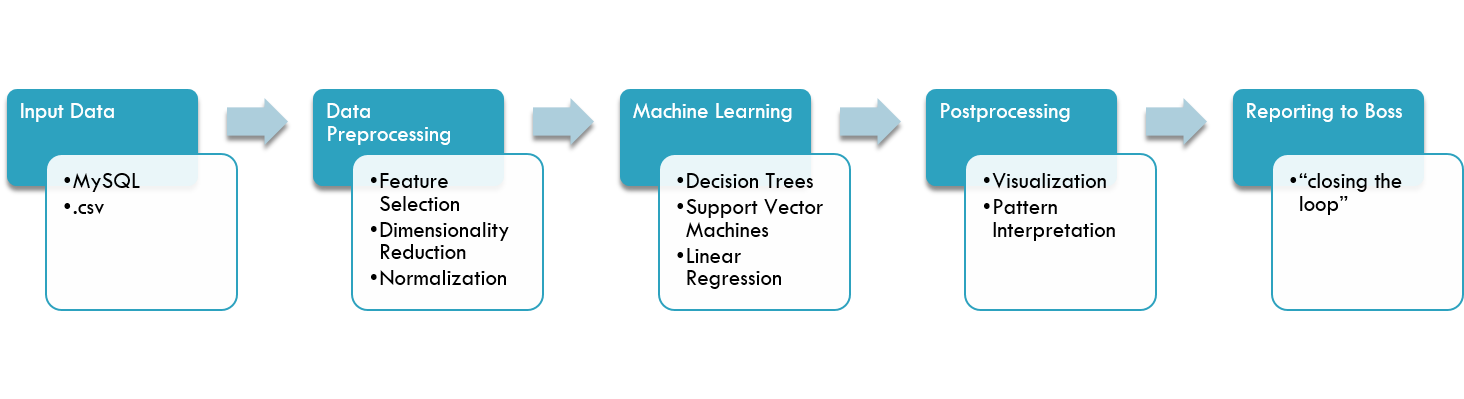
\includegraphics[width=\linewidth,keepaspectratio]{process}
%\end{center}
%\end{frame}
%
%%%%%%%%%%%%%%%%%%%%%%%%%%%%%%%%%%%%%%%%%%%%%%%%%%%%%%%%%%%%
%\begin{frame}[fragile]\frametitle{Data Mining/ Machine Learning Process}
%Transform raw input data into an appropriate format:
%	\begin{itemize}
%	\item Fusing data from multiple sources
%	\item Cleaning data to remove noise
%	\item Duplicate observations
%	\end{itemize}
%
%\end{frame}
%
%%%%%%%%%%%%%%%%%%%%%%%%%%%%%%%%%%%%%%%%%%%%%%%%%%%%%%%%%%%%
%\begin{frame}[fragile]\frametitle{Data Mining/ Machine Learning Process}
%\begin{itemize}
%\item Selecting relevant features
%\item Machine Learning
%\item Post Processing
%\begin{itemize}
%%\item Hypothesis testing to eliminate spurious data mining results
%\item Evaluation tests
%\item Visualization
%\end{itemize}
%\end{itemize}
%\end{frame}

%%%%%%%%%%%%%%%%%%%%%%%%%%%%%%%%%%%%%%%%%%%%%%%%%%%%%%%%%%%%
%\begin{frame}[fragile]\frametitle{The Learning Process}
%\begin{center}
%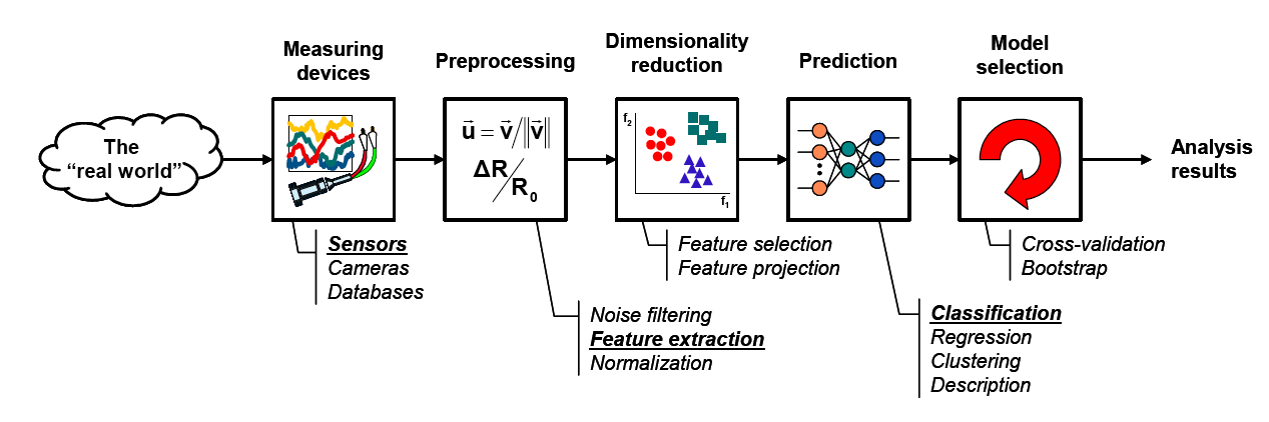
\includegraphics[width=\linewidth,keepaspectratio]{learning}
%\end{center}
%\end{frame}


%
%%%%%%%%%%%%%%%%%%%%%%%%%%%%%%%%%%%%%%%%%%%%%%%%%%%%%%%%%%%%
%\begin{frame}[fragile]\frametitle{Input Data}
%\begin{itemize}
%\item Available in data in variety of formats:
%	\begin{itemize}
%	\item Flat files (.csv or .txt)
%	\item Spreadsheets (Excel .xls tougher to deal with)
%	\item Relational tables (MySQL)
%	\item Text, data on web page (scraping necessary)
%	\end{itemize}
%\item Big Data / Data Warehouse
%\item Data spread out over multiple locations
%\item Present in
%	\begin{itemize}
%	\item Structured
%	\item Semi Structured
%	\item Unstructured
%	\end{itemize}
%\end{itemize}
%\end{frame}
%
%
%%%%%%%%%%%%%%%%%%%%%%%%%%%%%%%%%%%%%%%%%%%%%%%%%%%%
%\begin{frame}[fragile] \frametitle{(Big) Data Generation}
%
%\adjustbox{valign=t}{
%\begin{minipage}{0.45\linewidth}
%\begin{center}
%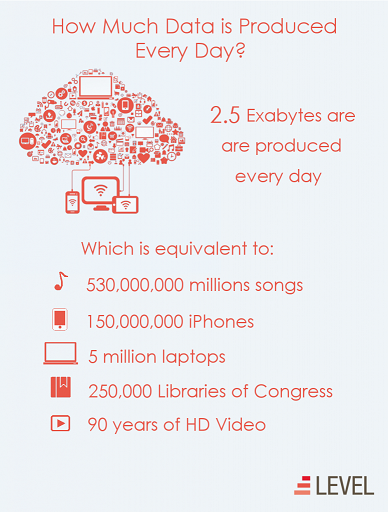
\includegraphics[width=\linewidth,keepaspectratio]{datagen}
%\end{center}
%\end{minipage}
%}
%\hfill
%\adjustbox{valign=t}{
%\begin{minipage}{0.45\linewidth}
%Some say that about 90\% of all the data in the world today has been created in the past few years. 
%
%\end{minipage}
%}
%{\tiny (http://www.northeastern.edu/levelblog/2016/05/13/how-much-data-produced-every-day/)}
%\end{frame}


%%%%%%%%%%%%%%%%%%%%%%%%%%%%%%%%%%%%%%%%%%%%%%%%%%%%%%%%%%%%
%\begin{frame}[fragile]\frametitle{Data Flow}
%\begin{itemize}
%\item To transform raw input data into an appropriate format for subsequent analysis:
%	\begin{itemize}
%	\item Fusing data from multiple sources
%	\item Cleaning data to remove noise
%	\item Duplicate observations
%	\end{itemize}
%\item Selecting records and features that are relevant to the data mining task at hand
%\item Machine Learning
%\item Post Processing
%\begin{itemize}
%\item Hypothesis testing to eliminate spurious data mining results
%\item Statistical significant tests, confidence intervals, 
%\item Visualization
%\end{itemize}
%\end{itemize}
%\end{frame}





%%%%%%%%%%%%%%%%%%%%%%%%%%%%%%%%%%%%%%%%%%%%%%%%%%%%%%%%%%%%
%\begin{frame}[fragile]\frametitle{Machine Learning Applications}
%\begin{itemize}
%\item Search on Google
%\item Face Recognition (Facebook)
%\item Classifier mail (Gmail)
%\item Spam recognition in Emails
%\item Robot Vision
%\item Character Recognition (OCR)
%\item Recommender Systems
%\item Feelings Analysis
%\end{itemize}
%\end{frame}

%
%%%%%%%%%%%%%%%%%%%%%%%%%%%%%%%%%%%%%%%%%%%%%%%%%%%%%%%%%%%%
%\begin{frame}[fragile]\frametitle{What is Machine Learning?}
%\begin{itemize}
%\item Humans learn from (past) experience
%\item Machines need to be told (instructions)
%\item Can we get computers to learn from experience (past data)? 
%\item YES. That's Machine Learning
%\end{itemize}
%\begin{center}
%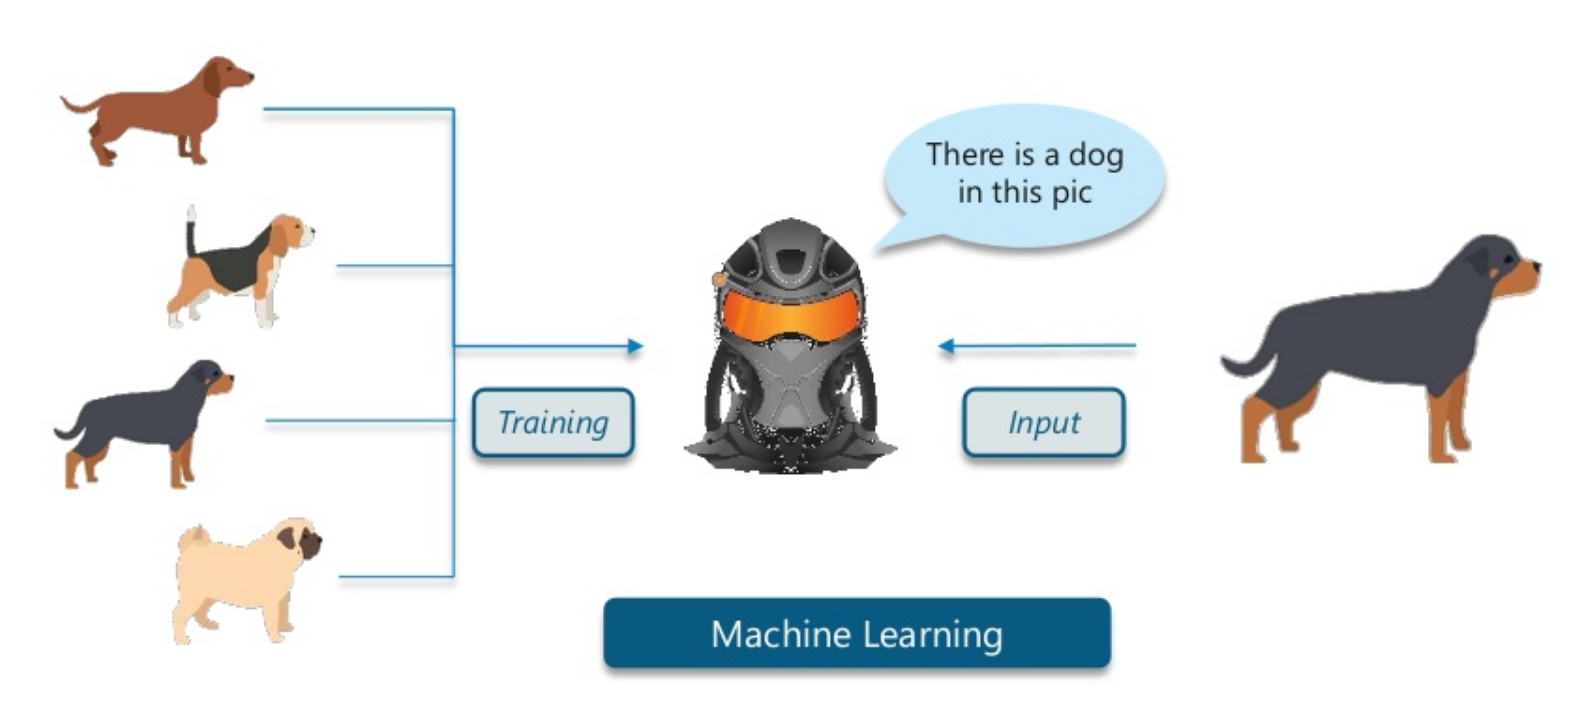
\includegraphics[width=\linewidth,keepaspectratio]{ml1}
%\end{center}
%\tiny{(Image Credit: A Gentle Introduction To Machine Learning; SciPy 2013 Presentation - Kastner, Kyle)}
%\end{frame}


% %%%%%%%%%%%%%%%%%%%%%%%%%%%%%%%%%%%%%%%%%%%%%%%%%%%%%%%%%%%%%%%%%%%%%%%%%%%%%%%%%%
% \begin{frame}[fragile]\frametitle{}
% \begin{center}
% {\Large Machine Learning Process}
% \end{center}
% \end{frame}



%%%%%%%%%%%%%%%%%%%%%%%%%%%%%%%%%%%%%%%%%%%%%%%%%%%%%%%%%%%%%%%%%%%%%%%%%%%%%%%%%%
\begin{frame}[fragile]\frametitle{}
\begin{center}
{\Large Types of Machine Learning}
\end{center}
\end{frame}


%%%%%%%%%%%%%%%%%%%%%%%%%%%%%%%%%%%%%%%%%%%%%%%%%%%%%%%%%%%
\begin{frame}[fragile]\frametitle{Two kinds of learning}
\begin{itemize}
\item Supervised
\item Unsupervised
\end{itemize}
\end{frame}


%%%%%%%%%%%%%%%%%%%%%%%%%%%%%%%%%%%%%%%%%%%%%%%%%%%%%%%%%%%
\begin{frame}[fragile]\frametitle{Supervised}
	\begin{itemize}
	\item Training data with correct answers
	\item Both used to train the model
	\item Then apply unseen data on model
	\end{itemize}
\end{frame}
%%%%%%%%%%%%%%%%%%%%%%%%%%%%%%%%%%%%%%%%%%%%%%%%%%%%%%%%%%%
\begin{frame}[fragile]\frametitle{Unsupervised}
	\begin{itemize}
	\item Training data with no answers
	\item Extract patterns, groups
	\end{itemize}	

\end{frame}

%%%%%%%%%%%%%%%%%%%%%%%%%%%%%%%%%%%%%%%%%%%%%%%%%%%%%%%%%%%
\begin{frame}[fragile]\frametitle{Some types of algorithms}
\begin{itemize}
\item Prediction: predicting a continuous variable from data
\item Classification: assigning records to predefined groups
\item Clustering: splitting records into groups based on similarity
\item Association learning: seeing what often appears together
\end{itemize}

\end{frame}

%%%%%%%%%%%%%%%%%%%%%%%%%%%%%%%%%%%%%%%%%%%%%%%%%%%%%%%%%%
\begin{frame}[fragile]\frametitle{Machine Learning Learning Algorithms}
\begin{center}
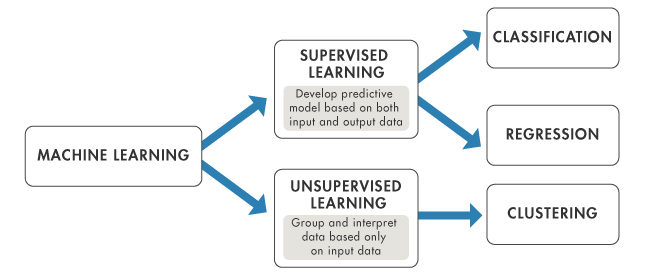
\includegraphics[width=\linewidth,keepaspectratio]{mlsupunsup}
\end{center}
\tiny{(Reference: Machine Learning in MATLAB - MATLAB \& Simulink - MathWorks)}
\end{frame}

%%%%%%%%%%%%%%%%%%%%%%%%%%%%%%%%%%%%%%%%%%%%%%%%%%%%%%%%%%
\begin{frame}[fragile]\frametitle{Machine Learning Learning Algorithms}

\begin{itemize}
\item Is this A or B? : Classification algorithms
\item Is this weird? : Anomaly detection algorithms
\item How much—or—How many? : Regression algorithms
\item How is this organized? : Clustering algorithms, Dimensionality reduction
\item What should I do next? : Reinforcement learning algorithms
\end{itemize}

\tiny{(Ref: Brandon Rohrer's breakdown of the ``5 questions data science answers'')}

\end{frame}

%%%%%%%%%%%%%%%%%%%%%%%%%%%%%%%%%%%%%%%%%%%%%%%%%%%%%%%%%%
\begin{frame}[fragile]\frametitle{Classification}
\begin{itemize}
\item \textbf{Description:} Identifying the category an object belongs to.
\item \textbf{Applications:} Spam detection, Image recognition.
\item \textbf{Algorithms:} SVM, nearest neighbors, random forest, Logistic Regression
\end{itemize}
\end{frame}


%%%%%%%%%%%%%%%%%%%%%%%%%%%%%%%%%%%%%%%%%%%%%%%%%%%%%%%%%%
\begin{frame}[fragile]\frametitle{Regression}
\begin{itemize}
\item \textbf{Description:} Predicting a continuous-valued attribute associated with an object.
\item \textbf{Applications:} Drug response, Stock prices.
\item \textbf{Algorithms:} Linear Regression 
\end{itemize}
\end{frame}

%%%%%%%%%%%%%%%%%%%%%%%%%%%%%%%%%%%%%%%%%%%%%%%%%%%%%%%%%%
\begin{frame}[fragile]\frametitle{Clustering}
\begin{itemize}
\item \textbf{Description:}Automatic grouping of similar objects into sets.
\item \textbf{Applications:} Customer segmentation, Grouping experiment outcomes
\item \textbf{Algorithms:} k-Means
\end{itemize}
\end{frame}

%%%%%%%%%%%%%%%%%%%%%%%%%%%%%%%%%%%%%%%%%%%%%%%%%%%%%%%%%%
\begin{frame}[fragile]\frametitle{Dimensionality Reduction}
\begin{itemize}
\item \textbf{Description: } Reducing the number of random variables to consider.
\item \textbf{Applications:} Visualization, Increased efficiency
\item \textbf{Algorithms:} PCA, Singular Value Decomposition 
\end{itemize}
\end{frame}

%%%%%%%%%%%%%%%%%%%%%%%%%%%%%%%%%%%%%%%%%%%%%%%%%%%%%%%%%%%
\begin{frame}[fragile]\frametitle{Popular Algorithms in Machine Learning}
	\begin{itemize}
	\item  Linear, Logistic Regression	
	\item  Decision Trees
	\item  SVM - Support Vector Machines, Naive Bayes
	\item K-Means
	\end{itemize}
%\begin{center}
%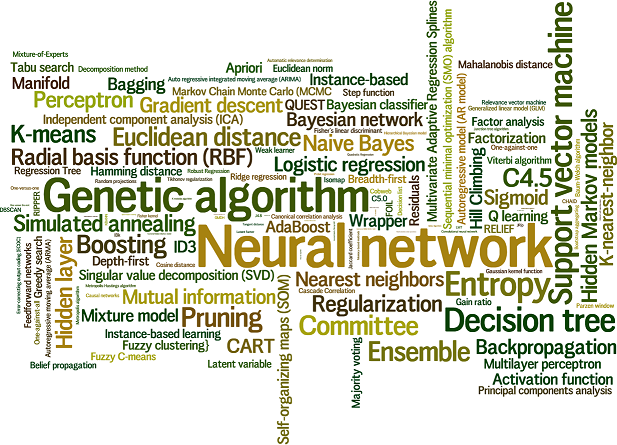
\includegraphics[width=0.6\linewidth,keepaspectratio]{mlalgos}
%\end{center}
%Which one is most suitable for the Housing price problem?
\end{frame}


%%%%%%%%%%%%%%%%%%%%%%%%%%%%%%%%%%%%%%%%%%%%%%%%%%%%%%%%%%%%%%
%%%\begin{frame}[fragile]\frametitle{Linear regression}
%%%	\begin{itemize}
%%%	\item  Attempts to find the ``best'' (generally straight) line
%%%	\item With one attribute (simple linear regression)
%%%	\item Combination of several (multiple linear regression)
%%%	\end{itemize}
%%%\end{frame}
%%%
%%%%%%%%%%%%%%%%%%%%%%%%%%%%%%%%%%%%%%%%%%%%%%%%%%%%%%%%%%%%%%
%%%\begin{frame}[fragile]\frametitle{Linear regression}
%%%\begin{center}
%%%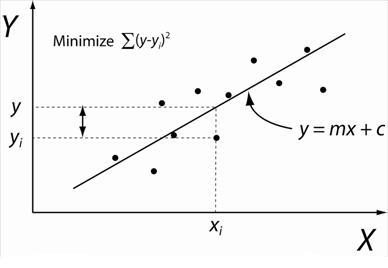
\includegraphics[width=0.8\linewidth,keepaspectratio]{linreg}
%%%\end{center}
%%%\end{frame}
%%%
%%%%%%%%%%%%%%%%%%%%%%%%%%%%%%%%%%%%%%%%%%%%%%%%%%%%%%%%%%%%%%%
%%%%\begin{frame}[fragile]\frametitle{Linear regression}
%%%%\begin{lstlisting}
%%%%import numpy as np
%%%%import matplotlib.pyplot as plt
%%%%
%%%%# Random data
%%%%N = 10
%%%%M = 2
%%%%input = np.random.random((N,M))
%%%%print input 
%%%%
%%%%# Setup matrices
%%%%m = np.shape(input)[0]
%%%%X = np.matrix([np.ones(m), input[:,0]]).T
%%%%y = np.matrix(input[:,1]).T
%%%%
%%%%# Solve for projection matrix
%%%%p_mat = np.linalg.inv(X.T.dot(X)).dot(X.T).dot(y)
%%%%print p_mat
%%%%
%%%%# Find regression line
%%%%xx = np.linspace(0, 1, 2)
%%%%yy = np.array(p_mat[0] + p_mat[1] * xx)
%%%%\end{lstlisting}
%%%%\end{frame}
%%%%
%%%%%%%%%%%%%%%%%%%%%%%%%%%%%%%%%%%%%%%%%%%%%%%%%%%%%%%%%%%%%%%
%%%%\begin{frame}[fragile]\frametitle{Linear regression}
%%%%%A particular run of this code generates the following input matrix:
%%%%%\begin{lstlisting}
%%%%%[[ 0.64840322  0.97285346]
%%%%% [ 0.77867147  0.87310339]
%%%%% [ 0.85072744  0.59023482]
%%%%% [ 0.3692784   0.59567815]
%%%%% [ 0.14654649  0.79422356]
%%%%% [ 0.46897942  0.06988269]
%%%%% [ 0.79239438  0.33157126]
%%%%% [ 0.88935174  0.04946074]
%%%%% [ 0.0615097   0.68082408]
%%%%% [ 0.63675227  0.93102028]]
%%%%%\end{lstlisting}
%%%%The values of which are the y-intercept and slope of the regression line, respectively:
%%%%\begin{lstlisting}
%%%%[[ 0.73461589]
%%%% [-0.25826794]]
%%%%\end{lstlisting}
%%%%\begin{center}
%%%%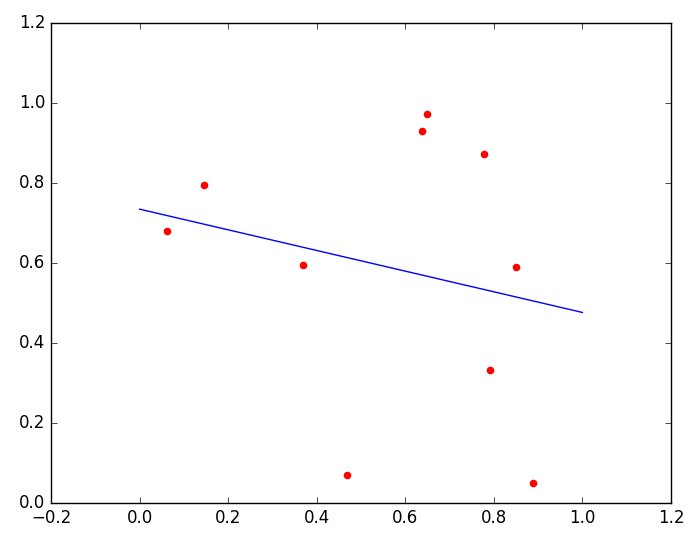
\includegraphics[width=0.6\linewidth,keepaspectratio]{linreg2}
%%%%\end{center}
%%%%\end{frame}
%%%
%%%%%%%%%%%%%%%%%%%%%%%%%%%%%%%%%%%%%%%%%%%%%%%%%%%%%%%%%%%%%%
%%%\begin{frame}[fragile]\frametitle{Decision Tree}
%%%	\begin{itemize}
%%%	\item  Type of flowchart for decision making process. 
%%%	\item Internal nodes represent tests on particular attributes,
%%%	\item Branches exiting nodes represent a single test outcome
%%%	\item Leaf nodes represent class labels.
%%%	\end{itemize}
%%%\end{frame}
%%%
%%%%%%%%%%%%%%%%%%%%%%%%%%%%%%%%%%%%%%%%%%%%%%%%%%%%%%%%%%%%%%
%%%\begin{frame}[fragile]\frametitle{Decision Tree}
%%%\begin{center}
%%%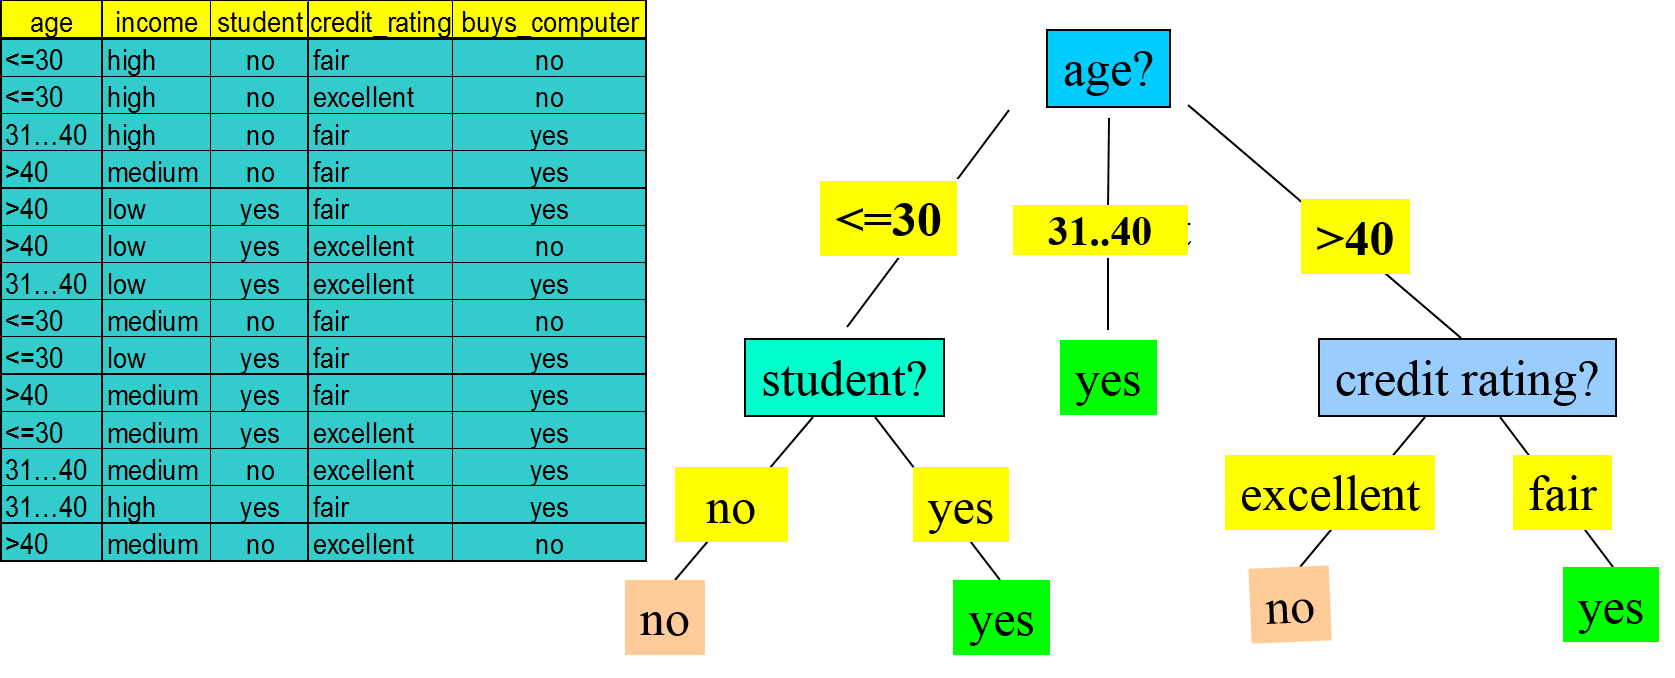
\includegraphics[width=\linewidth,keepaspectratio]{dectree2}
%%%\end{center}
%%%\end{frame}
%%%%%%%%%%%%%%%%%%%%%%%%%%%%%%%%%%%%%%%%%%%%%%%%%%%%%%%%%%%%%%%
%%%%\begin{frame}[fragile]\frametitle{Decision Tree}
%%%%	\begin{itemize}
%%%%	\item  While building our tree, the goal is to split on the attributes which create the purest child nodes possible, which would keep to a minimum the number
%%%%of splits that would need to be made in order to classify all instances in our dataset. 
%%%%\item This purity is generally measured by one of a number of different attribute selection measures.
%%%%	\end{itemize}
%%%%	\begin{center}
%%%%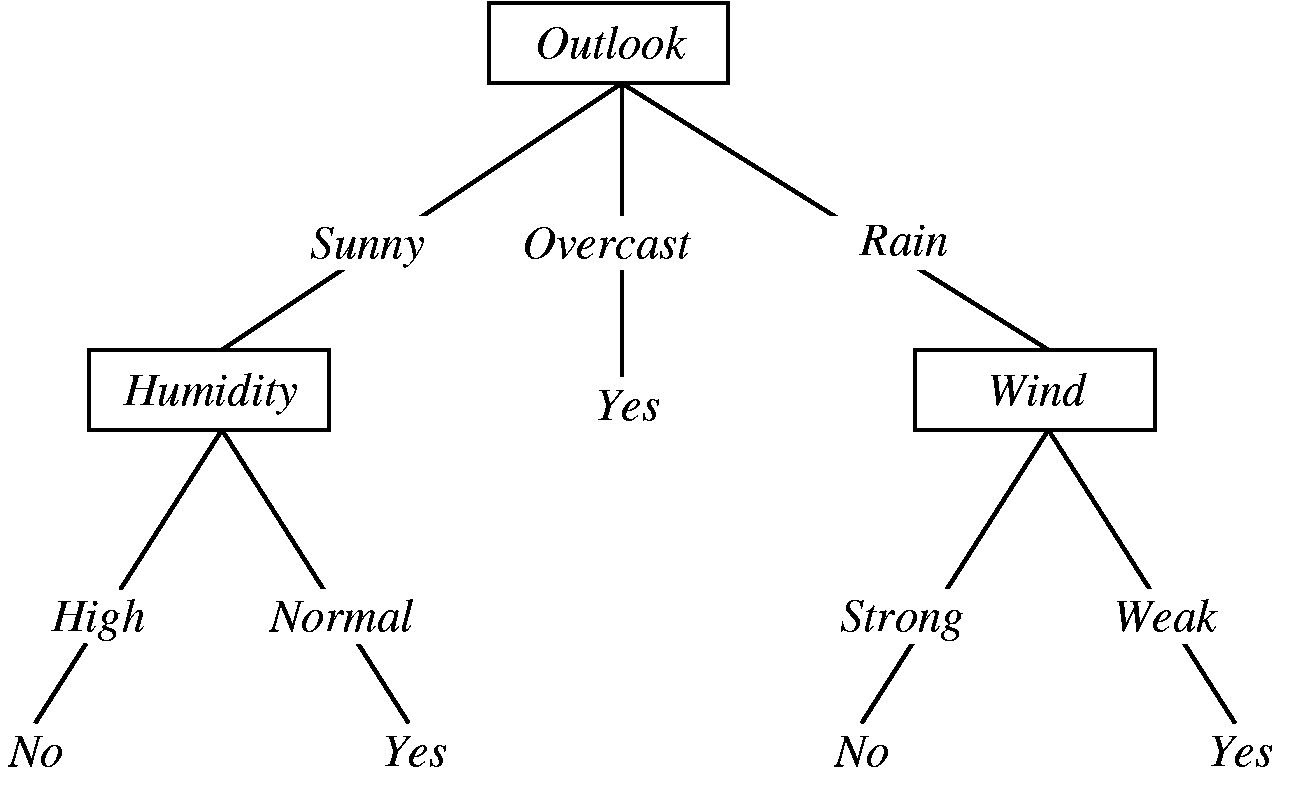
\includegraphics[width=0.6\linewidth,keepaspectratio]{dectree}
%%%%\end{center}
%%%%\end{frame}
%%%
%%%
%%%%%%%%%%%%%%%%%%%%%%%%%%%%%%%%%%%%%%%%%%%%%%%%%%%%%%%%%%%%%%
%%%\begin{frame}[fragile]\frametitle{Support Vector Machines}
%%%	\begin{itemize}
%%%	\item  Work by transforming into a higher dimension,
%%%	\item Optimal separation boundary
%%%	\item Can classify both linear and nonlinear data.
%%%	\item Not just for any separating hyperplane but the maximum-margin
%%%	\end{itemize}
%%%\end{frame}
%%%
%%%
%%%%%%%%%%%%%%%%%%%%%%%%%%%%%%%%%%%%%%%%%%%%%%%%%%%%%%%%%%%%%%
%%%\begin{frame}[fragile]\frametitle{Support Vector Machines}
%%%\begin{center}
%%%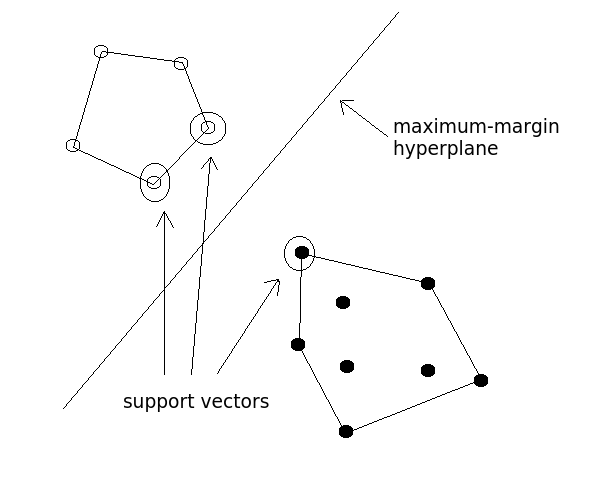
\includegraphics[width=0.8\linewidth,keepaspectratio]{svm}
%%%\end{center}
%%%\end{frame}
%%%
%%%%%%%%%%%%%%%%%%%%%%%%%%%%%%%%%%%%%%%%%%%%%%%%%%%%%%%%%%%%%%
%%%\begin{frame}[fragile]\frametitle{k-means Clustering}
%%%	\begin{itemize}
%%%	\item  k points are randomly chosen as centroids,
%%%	\item Added to the closest cluster. 
%%%	\item The centroids are re-calculated, all cluster membership is reset,
%%%	\item Iterates till no change to the centroids.
%%%	\end{itemize}
%%%\end{frame}
%%%
%%%
%%%%%%%%%%%%%%%%%%%%%%%%%%%%%%%%%%%%%%%%%%%%%%%%%%%%%%%%%%%%%%
%%%\begin{frame}[fragile]\frametitle{k-means Clustering}
%%%\begin{center}
%%%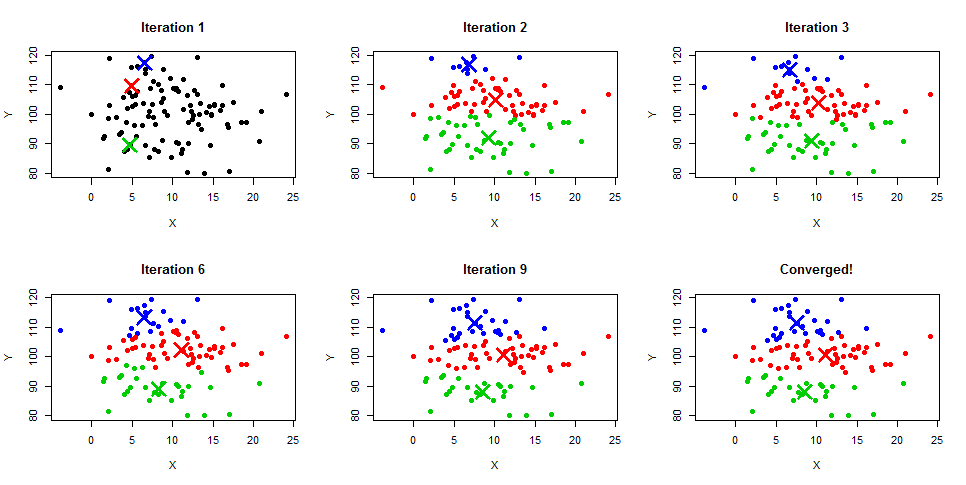
\includegraphics[width=\linewidth,keepaspectratio]{kmeans}
%%%\end{center}
%%%\end{frame}

%%%%%%%%%%%%%%%%%%%%%%%%%%%%%%%%%%%%%%%%%%%%%%%%%%%%%%%%%%%
\begin{frame}[fragile]\frametitle{Popular Algorithms in Machine Learning}
Recommendation: Is Gender the decider or Age?
\begin{center}
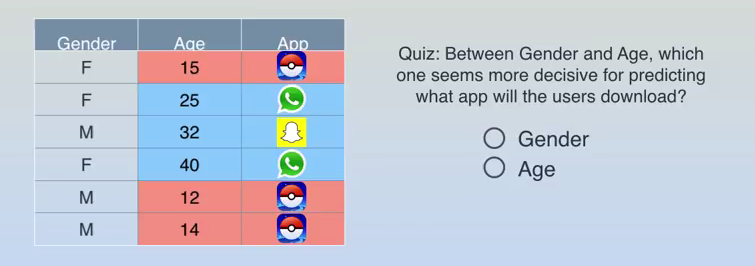
\includegraphics[width=\linewidth,keepaspectratio]{ml8}
\end{center}
Gender is not much, but all below 20 years downloaded Pokemon Go.Age splits data best.

\tiny{(Image Credit: A Gentle Introduction To Machine Learning; SciPy 2013 Presentation - Kastner, Kyle)}
\end{frame}

%%%%%%%%%%%%%%%%%%%%%%%%%%%%%%%%%%%%%%%%%%%%%%%%%%%%%%%%%%%
\begin{frame}[fragile]\frametitle{Popular Algorithms in Machine Learning}
Decision Tree.
\begin{center}
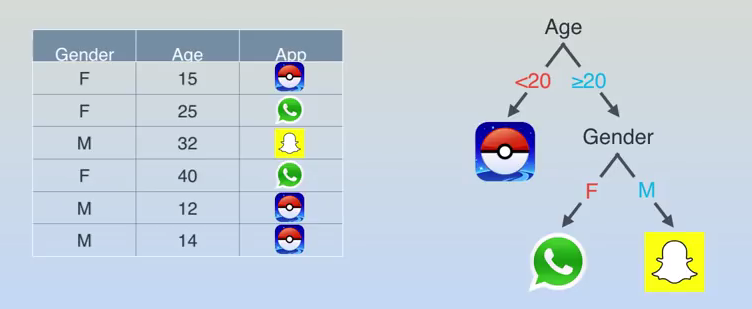
\includegraphics[width=\linewidth,keepaspectratio]{ml9}
\end{center}
Any new person can walk through the Tree and predict.

\tiny{(Image Credit: A Gentle Introduction To Machine Learning; SciPy 2013 Presentation - Kastner, Kyle)}
\end{frame}


%%%%%%%%%%%%%%%%%%%%%%%%%%%%%%%%%%%%%%%%%%%%%%%%%%%%%%%%%%%
\begin{frame}[fragile]\frametitle{Popular Algorithms in Machine Learning}
Deciding acceptance to Univ based on Test scores and grade.
\begin{center}
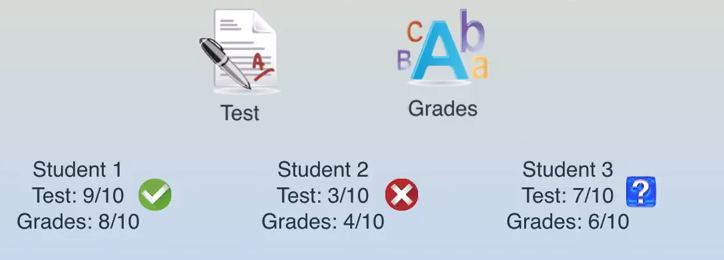
\includegraphics[width=\linewidth,keepaspectratio]{ml10}
\end{center}
Will Student 3 get accepted?

\tiny{(Image Credit: A Gentle Introduction To Machine Learning; SciPy 2013 Presentation - Kastner, Kyle)}
\end{frame}


%%%%%%%%%%%%%%%%%%%%%%%%%%%%%%%%%%%%%%%%%%%%%%%%%%%%%%%%%%%
\begin{frame}[fragile]\frametitle{Popular Algorithms in Machine Learning}
Putting it in a grid. Test score as X and Grades as Y. Prev data shown with acceptance colored.
\begin{center}
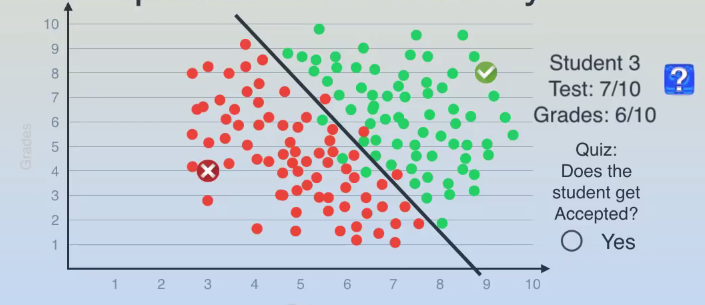
\includegraphics[width=\linewidth,keepaspectratio]{ml11}
\end{center}
After separating line, Student 3's fate can be predicted. That's Logistic Regression.

\tiny{(Image Credit: A Gentle Introduction To Machine Learning; SciPy 2013 Presentation - Kastner, Kyle)}
\end{frame}

%%%%%%%%%%%%%%%%%%%%%%%%%%%%%%%%%%%%%%%%%%%%%%%%%%%%%%%%%%%
\begin{frame}[fragile]\frametitle{Popular Algorithms in Machine Learning}
Which line separates best?
\begin{center}
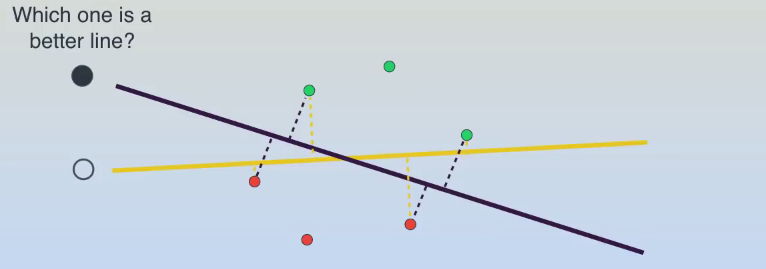
\includegraphics[width=\linewidth,keepaspectratio]{ml12}
\end{center}
The one with max separation in the middle. That's Support Vector Machine.

\tiny{(Image Credit: A Gentle Introduction To Machine Learning; SciPy 2013 Presentation - Kastner, Kyle)}

\end{frame}
%
%%%%%%%%%%%%%%%%%%%%%%%%%%%%%%%%%%%%%%%%%%%%%%%%%%%%%%%%%%%%
%\begin{frame}[fragile]\frametitle{Popular Algorithms in Machine Learning}
%Sometimes there is no separating line. 
%\begin{center}
%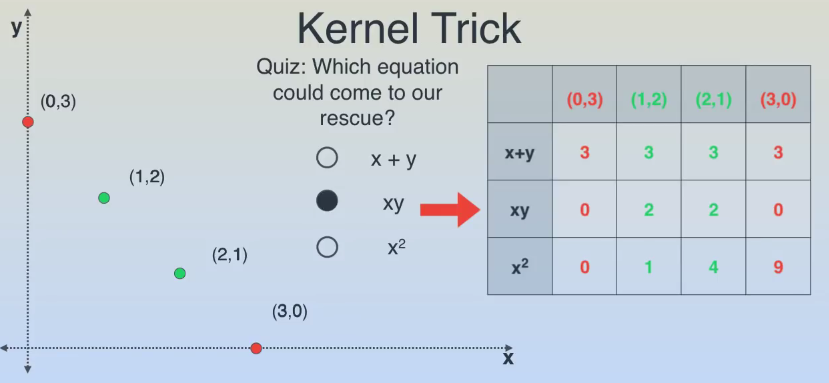
\includegraphics[width=\linewidth,keepaspectratio]{ml13}
%\end{center}
%Transform data and then find separating line/plane. xy gives 0 for red and 2 for green. That's Kernel Trick.
%
%\tiny{(Image Credit: A Gentle Introduction To Machine Learning; SciPy 2013 Presentation - Kastner, Kyle)}
%\end{frame}
%
%%%%%%%%%%%%%%%%%%%%%%%%%%%%%%%%%%%%%%%%%%%%%%%%%%%%%%%%%%%%
%\begin{frame}[fragile]\frametitle{Popular Algorithms in Machine Learning}
%$xy=1'$ separates $xy=0$ red points and $xy=2$ green points. Means $y=1/x$. Thats separating hyperbola.
%\begin{center}
%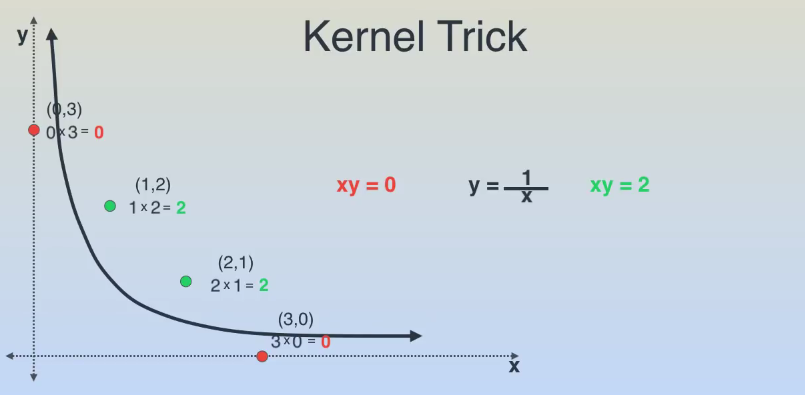
\includegraphics[width=\linewidth,keepaspectratio]{ml14}
%\end{center}
%
%\tiny{(Image Credit: A Gentle Introduction To Machine Learning; SciPy 2013 Presentation - Kastner, Kyle)}
%\end{frame}
%
%%%%%%%%%%%%%%%%%%%%%%%%%%%%%%%%%%%%%%%%%%%%%%%%%%%%%%%%%%%%
%\begin{frame}[fragile]\frametitle{Popular Algorithms in Machine Learning}
%Kernel Trick in 3D, with $z=xy$.
%\begin{center}
%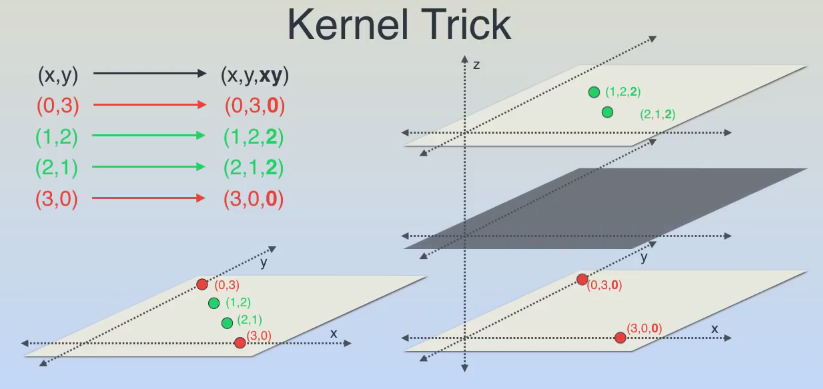
\includegraphics[width=\linewidth,keepaspectratio]{ml15}
%\end{center}
%\tiny{(Image Credit: A Gentle Introduction To Machine Learning; SciPy 2013 Presentation - Kastner, Kyle)}
%
%\end{frame}

%%%%%%%%%%%%%%%%%%%%%%%%%%%%%%%%%%%%%%%%%%%%%%%%%%%%%%%%%%%
\begin{frame}[fragile]\frametitle{Popular Algorithms in Machine Learning}
Classification: Detecting if mail is spam or not.
\begin{center}
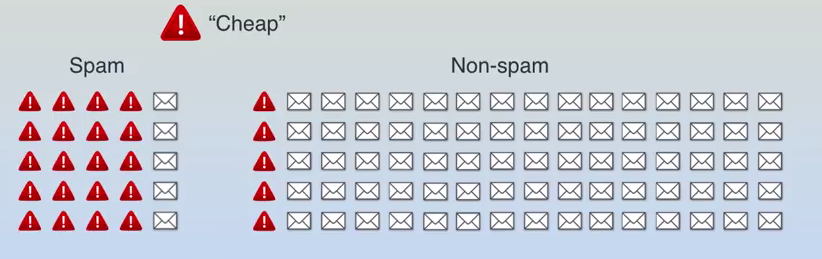
\includegraphics[width=\linewidth,keepaspectratio]{ml6}
\end{center}
Features: mail containing ``cheap''. 

Most past spam mails contain it.

\tiny{(Image Credit: A Gentle Introduction To Machine Learning; SciPy 2013 Presentation - Kastner, Kyle)}
\end{frame}

%%%%%%%%%%%%%%%%%%%%%%%%%%%%%%%%%%%%%%%%%%%%%%%%%%%%%%%%%%%
\begin{frame}[fragile]\frametitle{Popular Algorithms in Machine Learning}
Easy to compute probability of being a Spam, if it contains ``cheap''.
\begin{center}
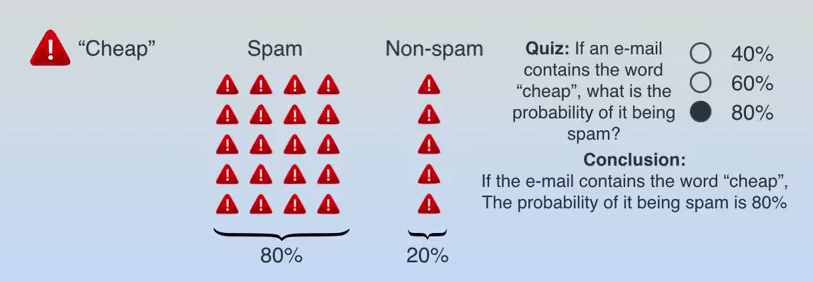
\includegraphics[width=\linewidth,keepaspectratio]{ml7}
\end{center}
That's Naive Bayes.

\tiny{(Image Credit: A Gentle Introduction To Machine Learning; SciPy 2013 Presentation - Kastner, Kyle)}
\end{frame}

%%%%%%%%%%%%%%%%%%%%%%%%%%%%%%%%%%%%%%%%%%%%%%%%%%%%%%%%%%%
\begin{frame}[fragile]\frametitle{Popular Algorithms in Machine Learning}
Wish to put 3 pizza shops in a city. Customers are plotted. What are the best locations?
\begin{center}
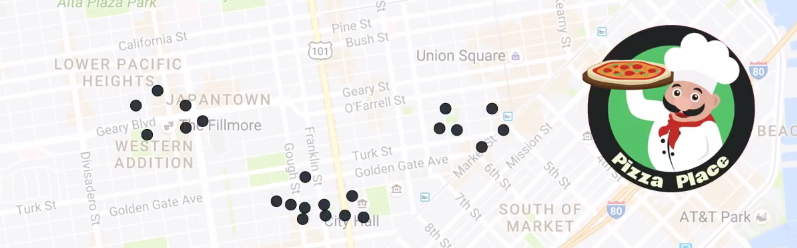
\includegraphics[width=\linewidth,keepaspectratio]{ml16}
\end{center}
Start with random locations and set ownership. Update locations. Repeat.
\end{frame}

%%%%%%%%%%%%%%%%%%%%%%%%%%%%%%%%%%%%%%%%%%%%%%%%%%%%%%%%%%%
\begin{frame}[fragile]\frametitle{Popular Algorithms in Machine Learning}
Locations settle at the centroids of the clusters.
\begin{center}
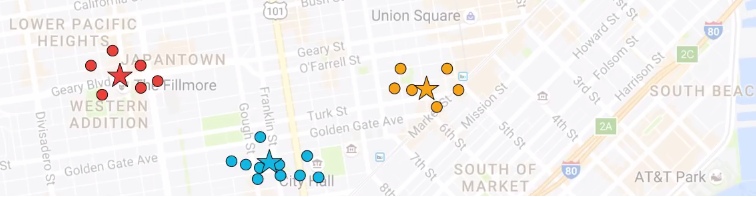
\includegraphics[width=\linewidth,keepaspectratio]{ml17}
\end{center}
That's K-means.

\tiny{(Image Credit: A Gentle Introduction To Machine Learning; SciPy 2013 Presentation - Kastner, Kyle)}
\end{frame}



%%%%%%%%%%%%%%%%%%%%%%%%%%%%%%%%%%%%%%%%%%%%%%%%%%%%%%%%%%%%%
%%%\begin{frame}[fragile]\frametitle{Trade-Off Between Model Flexibility and Interpret-ability}
%%%\begin{itemize}
%%%\item Some models (e.g. linear) are less flexible and more restrictive.
%%%\item Q: Why would one choose restrictive method than flexible?
%%%\item A: For inference, restrictive models are more interpretable. In linear model, it is easy to understand relationship between Y and X1, X2, \ldots
%%%\item For prediction, we might only be interested in accuracy and not the interpretability of the model
%%%\end{itemize}
%%%\begin{center}
%%%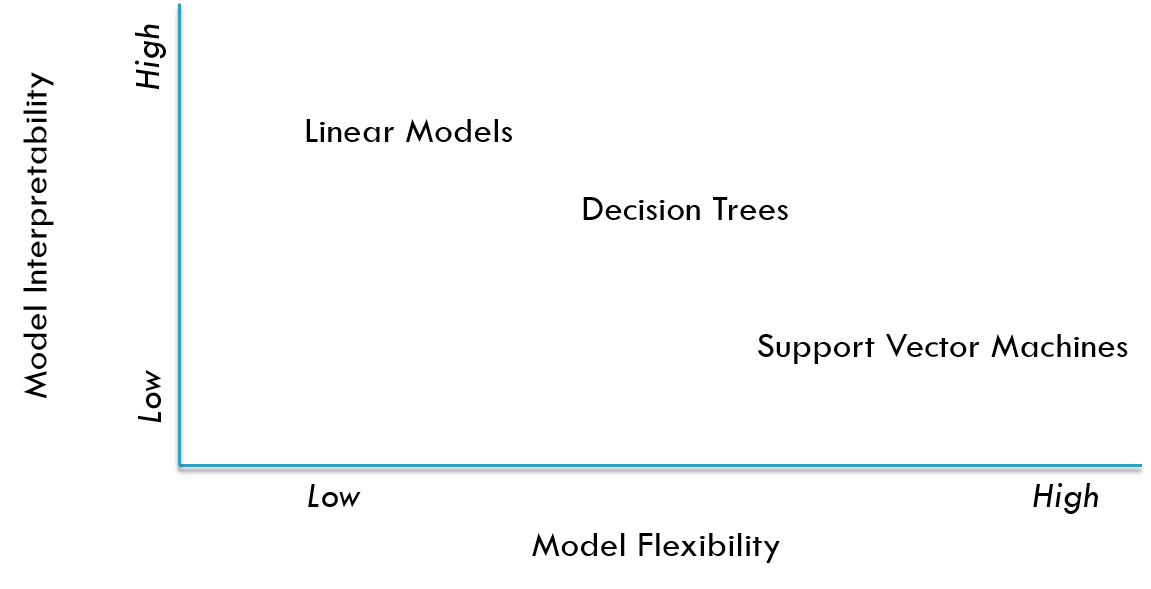
\includegraphics[width=0.5\linewidth,keepaspectratio]{models}
%%%\end{center}
%%%\end{frame}
%%
%%%
%%%%%%%%%%%%%%%%%%%%%%%%%%%%%%%%%%%%%%%%%%%%%%%%%%%%%%%%%%%%%
%%%\begin{frame}[fragile]\frametitle{Evaluation}
%%%Model Evaluation on Test Set (Regression) - Mean Squared Error
%%%\begin{itemize}
%%%\item Mean Squared Error: measuring the ``quality of fit''
%%%\item Will be small if the predicted responses are very close to the true responses
%%%$MSE = \frac{1}{n} \sum (y_i - f(x_i))^2$
%%%\end{itemize}
%%%\end{frame}
%%
%%%%%%%%%%%%%%%%%%%%%%%%%%%%%%%%%%%%%%%%%%%%%%%%%%%%%%%%%%%%%
%%%\begin{frame}[fragile]\frametitle{Example: Churn Dataset}
%%%
%%%\begin{itemize}
%%%\item From UCI Machine Learning Repository
%%%\item \url{http://taz.cs.wcupa.edu/~rburns/DataMining/datasets/churn.txt}
%%%\item 3333 records (customers)
%%%\item 20 predictor variables
%%%\item 1 target variable: churn (whether or not customer left the company)
%%%\end{itemize}
%%%\end{frame}
%%%
%%%%%%%%%%%%%%%%%%%%%%%%%%%%%%%%%%%%%%%%%%%%%%%%%%%%%%%%%%%%%
%%%\begin{frame}[fragile]\frametitle{Churn variables}
%%%\small
%%%\adjustbox{valign=t}{
%%%\begin{minipage}{0.45\linewidth}
%%%
%%%\begin{itemize}
%%%\item State: categorical (50 states + DC)
%%%\item Account Length: integer (how long account has been active)
%%%\item Area Code: categorical
%%%\item Phone Number: (can be used for customer ID)
%%%\item International Plan: binary (yes or no)
%%%\item Voice Mail Plan: binary
%%%\item Number of Voice Mail Messages: integer
%%%\item Total Day Minutes: continuous (minutes of day calls by customer)
%%%\item Total Day Calls: integer
%%%\item Total Day Charge: continuous
%%%\end{itemize}
%%%
%%%\end{minipage}
%%%}
%%%\hfill
%%%\adjustbox{valign=t}{
%%%\begin{minipage}{0.45\linewidth}
%%%
%%%\begin{itemize}
%%%\item Total Evening Minutes
%%%\item Total Evening Calls
%%%\item Total Evening Charge
%%%\item Total Night Minutes
%%%\item Total Night Calls
%%%\item Total Night Charge
%%%\item Total International Minutes
%%%\item Total International Calls
%%%\item Total International Charge
%%%\item Number of Calls to Customer Server: integer
%%%\item Churn: binary (whether or not customer has left the company)
%%%\end{itemize}
%%%
%%%\end{minipage}
%%%}
%%%\end{frame}
%%%
%%%%%%%%%%%%%%%%%%%%%%%%%%%%%%%%%%%%%%%%%%%%%%%%%%%%%%%%%%%%%
%%%\begin{frame}[fragile]\frametitle{Desired Results}
%%%\begin{itemize}
%%%\item Would like our findings from analyzing the Churn dataset to be applicable to all customers (the population), not just the subset of 3333 customers in the dataset (the sample).
%%%\item Sample needs to be representative of the population. If not, (sample characteristics deviate systematically from the population characteristics), statistical inference should not be applied.
%%%\end{itemize}
%%%\end{frame}
%%%
%%%%%%%%%%%%%%%%%%%%%%%%%%%%%%%%%%%%%%%%%%%%%%%%%%%%%%%%%%%%%
%%%\begin{frame}[fragile]\frametitle{Vocabulary}
%%%\begin{itemize}
%%%\item Parameter: a characteristic of the population. Example: mean number of customer service calls, of all phone customers
%%%\item Statistic: a characteristic of the sample. Example: mean number of customer service calls, for customers in the sample. 3333 customers in Churn sample, mean is 1.563. ???? Customers in population, mean is ????
%%%\item Values of population parameters are usually unknown.
%%%\end{itemize}
%%%\begin{center}
%%%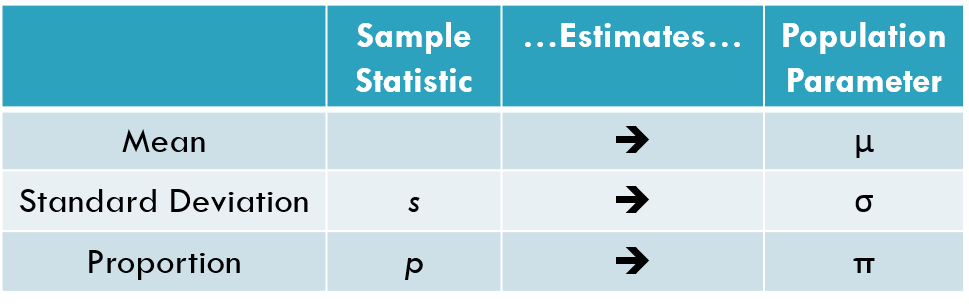
\includegraphics[width=0.8\linewidth,keepaspectratio]{symbols}
%%%\end{center}
%%%\end{frame}
%%%
%%%%%%%%%%%%%%%%%%%%%%%%%%%%%%%%%%%%%%%%%%%%%%%%%%%%%%%%%%%%%
%%%\begin{frame}[fragile]\frametitle{Estimation}
%%%\begin{itemize}
%%%\item Point Estimation: the use of a single known value of a statistic to estimation the population parameter. Examples: Using sample mean to estimate the population mean
%%%\item How confident are we in our estimates? Point estimates have no measure of confidence in their accuracy
%%%\item How close is the point estimate? Point estimates will ``almost always'' have some error: sampling error
%%%\end{itemize}
%%%\end{frame}
%%%
%%%
%%%%%%%%%%%%%%%%%%%%%%%%%%%%%%%%%%%%%%%%%%%%%%%%%%%%%%%%%%%%%
%%%\begin{frame}[fragile]\frametitle{Confidence Interval Estimation}
%%%\begin{itemize}
%%%\item Confidence Interval Estimate: interval produced from a point estimate, with an associated confidence level specifying the probability that the interval contains the parameter
%%%\item General Form: $Point Estimate \pm  MarginOfError$
%%%``margin of error'' as a measure of precision for the estimate
%%%\item t-interval for the population mean: $\bar{x} \pm t_{\alpha/2}(\frac{s}{\sqrt n})$
%%%\item t-interval may be used, when either:Population is normal, Sample size is large
%%%\item 95\% confidence level: $\alpha=1-.95=.05$
%%%\end{itemize}
%%%\end{frame}
%%%
%%%
%%%%%%%%%%%%%%%%%%%%%%%%%%%%%%%%%%%%%%%%%%%%%%%%%%%%%%%%%%%%%
%%%\begin{frame}[fragile]\frametitle{Examples}
%%%\begin{itemize}
%%%\item 95\% t-interval for the mean number of customer service calls for all customers:
%%%\item $\bar{x} \pm t_{\alpha/2}(\frac{s}{\sqrt n})$
%%%\item $1.563 \pm 1.96(\frac{1.315}{\sqrt 3333})$
%%%\item $1.563 \pm 0.045$
%%%\item $(1.518,1.608)$
%%%\end{itemize}
%%%\end{frame}
%%%
%%%
%%%%%%%%%%%%%%%%%%%%%%%%%%%%%%%%%%%%%%%%%%%%%%%%%%%%%%%%%%%%%
%%%\begin{frame}[fragile]\frametitle{Examples}
%%%\begin{itemize}
%%%\item Let's only select customers who have: Enrolled in the International Plan, Enrolled in the VoiceMail Plan, $\ge 200$ day minutes
%%%\item Reduces sample from 3333 to 28 customers. Still large enough to construct the confidence interval
%%%\item $\bar{x} \pm t_{\alpha/2}(\frac{s}{\sqrt n})$
%%%\item $1.607 \pm 2.051(\frac{1.892}{\sqrt 28})$
%%%\item $1.607 \pm 0.733$
%%%\item $(0.874,2.34)$
%%%\end{itemize}
%%%\end{frame}
%%
%%



%%%%%%%%%%%%%%%%%%%%%%%%%%%%%%%%%%%%%%%%%%%%%%%%%%%%%%%%%%%%
%\begin{frame}[fragile]\frametitle{Machine Learning}
%\begin{center}
%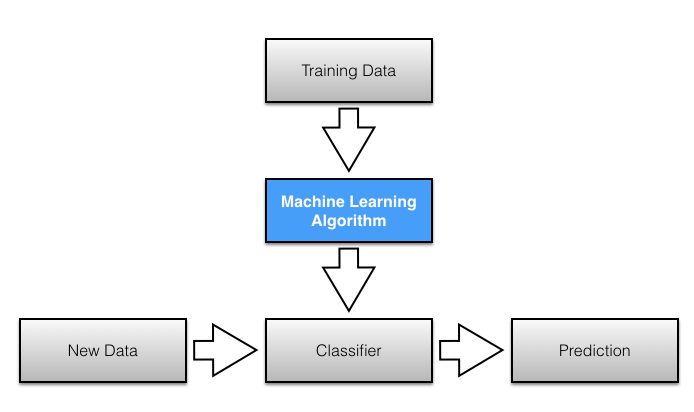
\includegraphics[width=0.8\linewidth,keepaspectratio]{mldef}
%\end{center}
%	\begin{itemize}
%	\item Supervised: with training data
%	\item Unsupervised: with training data without lables/outcome
%	\end{itemize}
%	
%\end{frame}
%
%%%%%%%%%%%%%%%%%%%%%%%%%%%%%%%%%%%%%%%%%%%%%%%%%%%%%%%%%%%%
%\begin{frame}[fragile]\frametitle{Supervised Learning}
%\begin{center}
%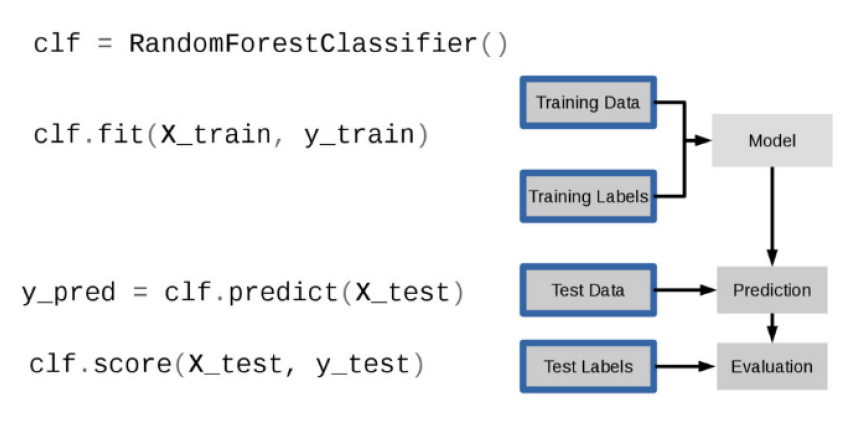
\includegraphics[width=\linewidth,keepaspectratio]{suplearn}
%\end{center}
%\end{frame}
%
%%%%%%%%%%%%%%%%%%%%%%%%%%%%%%%%%%%%%%%%%%%%%%%%%%%%%%%%%%%%
%\begin{frame}[fragile]\frametitle{Unsupervised Learning}
%\begin{center}
%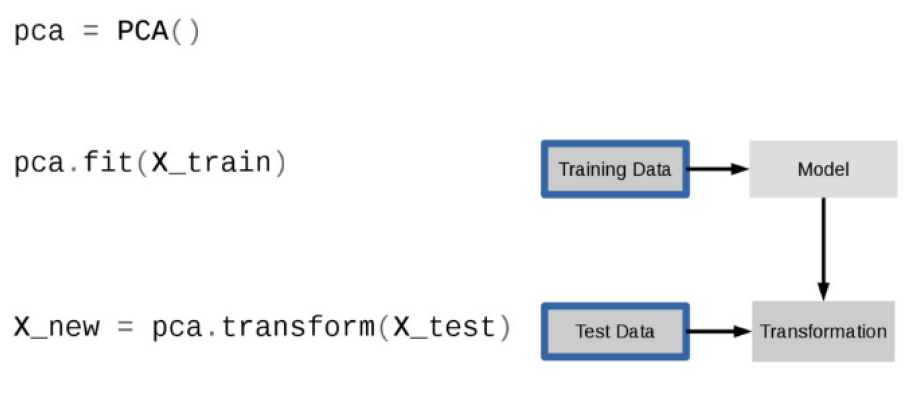
\includegraphics[width=\linewidth,keepaspectratio]{unsuplearn}
%\end{center}
%\end{frame}
%
%
%
%
%%%%%%%%%%%%%%%%%%%%%%%%%%%%%%%%%%%%%%%%%%%%%%%%%%%%%%%%%%%%
%\begin{frame}[fragile]\frametitle{Example}
%Predicting price of the third house looking at past house prices
%\begin{center}
%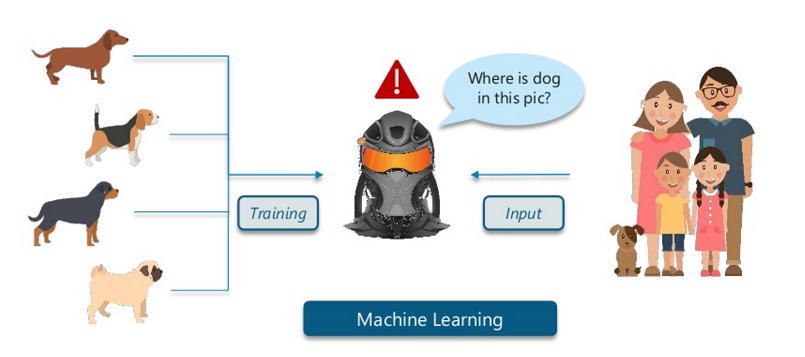
\includegraphics[width=\linewidth,keepaspectratio]{ml2}
%\end{center}
%\tiny{(Image Credit: A Gentle Introduction To Machine Learning; SciPy 2013 Presentation - Kastner, Kyle)}
%\end{frame}
%
%%%%%%%%%%%%%%%%%%%%%%%%%%%%%%%%%%%%%%%%%%%%%%%%%%%%%%%%%%%%
%\begin{frame}[fragile]\frametitle{What is Machine Learning?}
%Fit line and answer.
%\begin{center}
%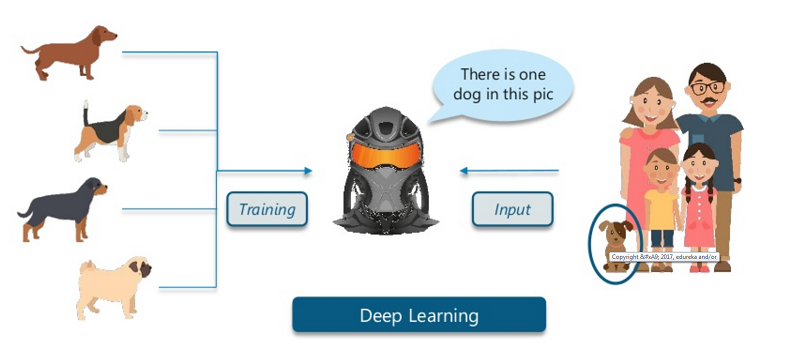
\includegraphics[width=\linewidth,keepaspectratio]{ml3}
%\end{center}
%Called Linear Regression!!
%
%\tiny{(Image Credit: A Gentle Introduction To Machine Learning; SciPy 2013 Presentation - Kastner, Kyle)}
%\end{frame}
%
%%%%%%%%%%%%%%%%%%%%%%%%%%%%%%%%%%%%%%%%%%%%%%%%%%%%%%%%%%%%
%\begin{frame}[fragile]\frametitle{What is Machine Learning?}
%How to find best fitting line. The one with minimum error.
%\begin{center}
%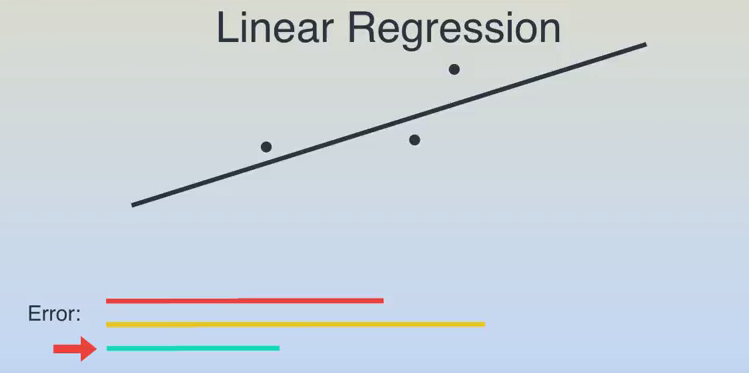
\includegraphics[width=\linewidth,keepaspectratio]{ml4}
%\end{center}
%How to find minimum error line?
%
%\tiny{(Image Credit: A Gentle Introduction To Machine Learning; SciPy 2013 Presentation - Kastner, Kyle)}
%\end{frame}
%
%%%%%%%%%%%%%%%%%%%%%%%%%%%%%%%%%%%%%%%%%%%%%%%%%%%%%%%%%%%%
%\begin{frame}[fragile]\frametitle{What is Machine Learning?}
%Optimization: Form error equation based on slope.
%\begin{center}
%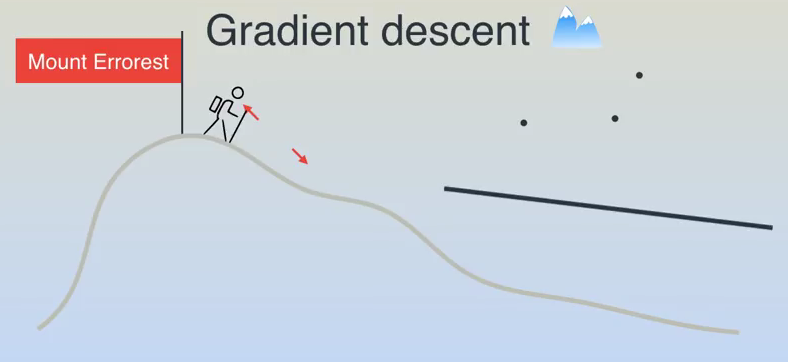
\includegraphics[width=\linewidth,keepaspectratio]{ml5}
%\end{center}
%Get slope at min Error. Thats the best line.
%
%\tiny{(Image Credit: A Gentle Introduction To Machine Learning; SciPy 2013 Presentation - Kastner, Kyle)}
%\end{frame}
%

%%%%%%%%%%%%%%%%%%%%%%%%%%%%%%%%%%%%%%%%%%%%%%%%%%%%%%%%%%%%%%%%%%%%%%%%%%%%%%%%%%
\begin{frame}[fragile]\frametitle{}
\begin{center}
{\Large Example: Predicting House Price}
\end{center}

{\tiny (Ref: Machine Learning is Fun! - Adam Geitgey)}
\end{frame}

%%%%%%%%%%%%%%%%%%%%%%%%%%%%%%%%%%%%%%%%%%%%%%%%%%%%%%%%%%%
\begin{frame}[fragile]\frametitle{Numerical way}
\begin{center}
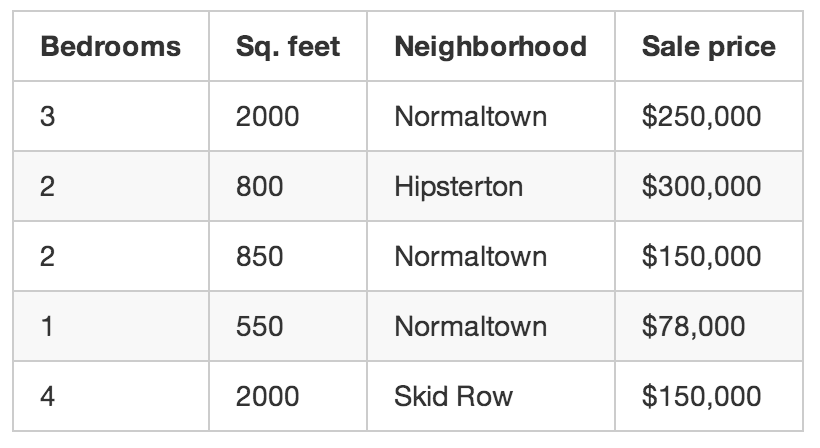
\includegraphics[width=0.6\linewidth,keepaspectratio]{housing1}
\end{center}
\begin{center}
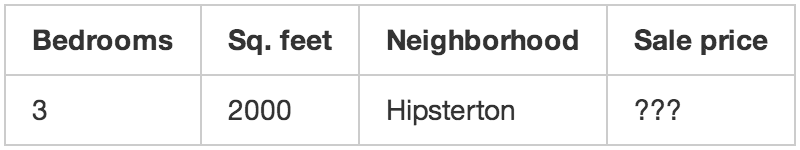
\includegraphics[width=0.6\linewidth,keepaspectratio]{housing2}
\end{center}
\end{frame}

%%%%%%%%%%%%%%%%%%%%%%%%%%%%%%%%%%%%%%%%%%%%%%%%%%%%%%%%%%%
\begin{frame}[fragile]\frametitle{Machine Learning Type}
\begin{itemize}
\item This is supervised learning. 
\item Knew how much each house sold for, 
\item So, knew the answer to the problem 
\item Need work backwards to figure out the logic.
\end{itemize}
\end{frame}

%
%%%%%%%%%%%%%%%%%%%%%%%%%%%%%%%%%%%%%%%%%%%%%%%%%%%%%%%%%%%%
%\begin{frame}[fragile]\frametitle{Unsupervised Learning}
%What if you didn't know the sale price for each house? Even if all you know is the size, location, etc of each house, it turns out you can still do some really cool stuff. This is called unsupervised learning.
%\begin{center}
%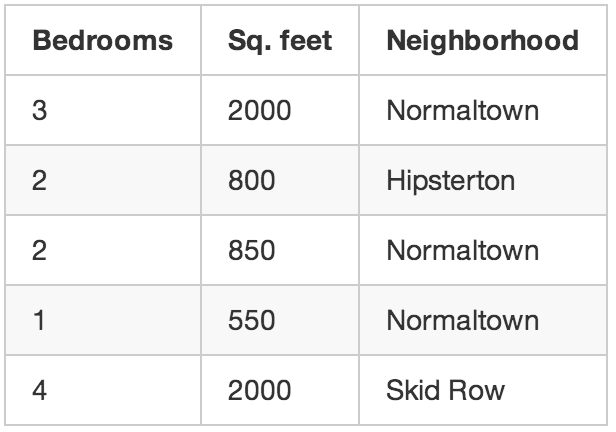
\includegraphics[width=0.6\linewidth,keepaspectratio]{housing3}
%\end{center}
%
%
%\end{frame}
%
%%%%%%%%%%%%%%%%%%%%%%%%%%%%%%%%%%%%%%%%%%%%%%%%%%%%%%%%%%%%
%\begin{frame}[fragile]\frametitle{Unsupervised Learning}
%	\begin{itemize}
%	\item You could have an algorithm that automatically identified different market segments in your data.
%	\item you could do is automatically identify any outlier houses that were way different than everything else. Maybe those outlier houses are giant mansions and you can focus your best sales people on those areas because they have bigger commissions.
%	\end{itemize}
%\end{frame}

%%%%%%%%%%%%%%%%%%%%%%%%%%%%%%%%%%%%%%%%%%%%%%%%%%%%%%%%%%%
\begin{frame}[fragile]\frametitle{Traditional way}
\begin{lstlisting}
def estimate_house_sales_price(num_of_bedrooms, sqft, neighborhood):
	price = 0
	price_per_sqft = 200

 	if neighborhood == "hipsterton": 
 		price_per_sqft = 400
	elif neighborhood == "skid row": 
		price_per_sqft = 100
	
	price = price_per_sqft * sqft
	if num_of_bedrooms == 0: 
		price = price - 20000
	else: 
		price = price + (num_of_bedrooms * 1000)
    
	return price
\end{lstlisting}
BUT, how to decide which numbers to put? PRAY!!!
\end{frame}

%%%%%%%%%%%%%%%%%%%%%%%%%%%%%%%%%%%%%%%%%%%%%%%%%%%%%%%%%%%
\begin{frame}[fragile]\frametitle{Prayer}
	\begin{itemize}
	\item Wouldn't it be better if computer figures out? 
	\item Treat it as black box
	\item Feed Inputs and outputs
	\item That's it!!
	\end{itemize}
\begin{lstlisting}
def estimate_house_sales_price(num_of_bedrooms, sqft, neighborhood):
    price = <computer, plz do some math for me>
    return price
\end{lstlisting}
\end{frame}


%%%%%%%%%%%%%%%%%%%%%%%%%%%%%%%%%%%%%%%%%%%%%%%%%%%%%%%%%%%
\begin{frame}[fragile]\frametitle{Prayer granted!!}
\begin{lstlisting}
def estimate_house_sales_price(num_of_bedrooms, sqft, neighborhood):
	price = 0
	price += num_of_bedrooms * .841
	price += sqft * 1231.123
	price += neighborhood * 2.324
	price += 201.234
	return price
\end{lstlisting}
	\begin{itemize}
	\item Notice the magic numbers
	\item .841, 1231.123, 2.324, and 201.234. 
	\item These are weights. 
	\item Better the weights - better the prediction!
	\item Done!!
	\end{itemize}
\end{frame}

%%%%%%%%%%%%%%%%%%%%%%%%%%%%%%%%%%%%%%%%%%%%%%%%%%%%%%%%%%%
\begin{frame}[fragile]\frametitle{How to figure out? A dumb way}
Step 1: Start with each weight set to 1.0:
\begin{lstlisting}
def estimate_house_sales_price(num_of_bedrooms, sqft, neighborhood):
	price = 0
	price += num_of_bedrooms * 1.0
	price += sqft * 1.0
	price += neighborhood * 1.0
	price += 1.0
	return price
\end{lstlisting}
\end{frame}

%%%%%%%%%%%%%%%%%%%%%%%%%%%%%%%%%%%%%%%%%%%%%%%%%%%%%%%%%%%
\begin{frame}[fragile]\frametitle{How to figure out? A dumb way}
Step 2: Guess/predict for all houses 
\begin{center}
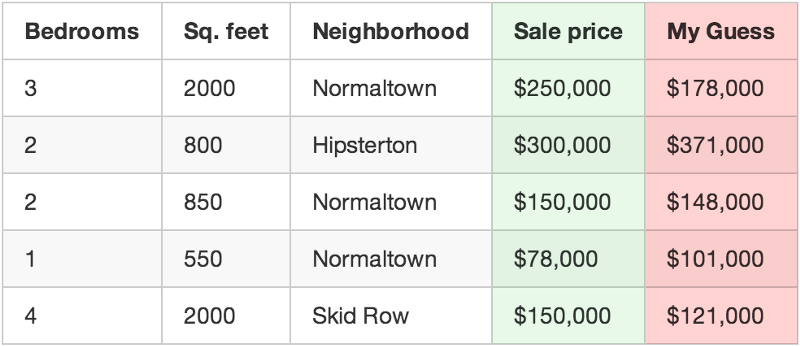
\includegraphics[width=0.8\linewidth,keepaspectratio]{housing4}
\end{center}
Predictions NOT good, right?
\end{frame}

%%%%%%%%%%%%%%%%%%%%%%%%%%%%%%%%%%%%%%%%%%%%%%%%%%%%%%%%%%%
\begin{frame}[fragile]\frametitle{What to do?}
	\begin{itemize}
	\item Actual \$250,000, but guessed \$178,000
	\item Off by \$72,000 for that single house.
	\item Diff can be positive or negative, so square it
	\item Add squared diffs of all houses.
	\item Total: \$86,123,373. 
	\item Thats whole error in the system.
	\item That's how ``wrong'' your function currently is.
	\end{itemize}
\end{frame}

%%%%%%%%%%%%%%%%%%%%%%%%%%%%%%%%%%%%%%%%%%%%%%%%%%%%%%%%%%%
\begin{frame}[fragile]\frametitle{What Next?}
	\begin{itemize}
	\item Average per house error is ``cost''.
	\item Get cost to be zero by playing with the weights. 
	\item Thats the Goal!!!
	\end{itemize}
\end{frame}

%%%%%%%%%%%%%%%%%%%%%%%%%%%%%%%%%%%%%%%%%%%%%%%%%%%%%%%%%%%
\begin{frame}[fragile]\frametitle{Mathematically}
\begin{center}
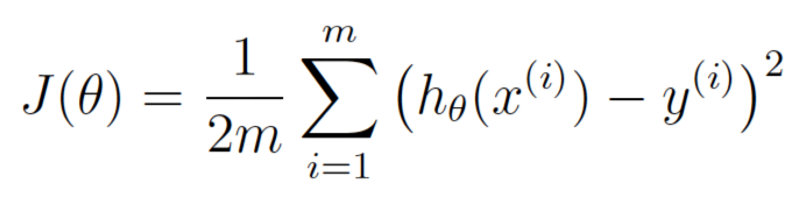
\includegraphics[width=0.8\linewidth,keepaspectratio]{costeqn}
\end{center}
\end{frame}

%%%%%%%%%%%%%%%%%%%%%%%%%%%%%%%%%%%%%%%%%%%%%%%%%%%%%%%%%%%
\begin{frame}[fragile]\frametitle{Graphically}
Plotting cost values,  for all possible ranges of weights for number\_of\_bedrooms and sqft:
\begin{center}
\includegraphics[width=0.8\linewidth,keepaspectratio]{costgrph}
\end{center}
\end{frame}

%%%%%%%%%%%%%%%%%%%%%%%%%%%%%%%%%%%%%%%%%%%%%%%%%%%%%%%%%%%
\begin{frame}[fragile]\frametitle{Graphically}
Cost is lowest at lowest point of the surface. Ideal.

Weights at that point are the answers!
\begin{center}
\includegraphics[width=0.8\linewidth,keepaspectratio]{costgrph1}
\end{center}
\end{frame}


%%%%%%%%%%%%%%%%%%%%%%%%%%%%%%%%%%%%%%%%%%%%%%%%%%%%%%%%%%%
\begin{frame}[fragile]\frametitle{How to find the lowest cost point?}
	\begin{itemize}
	\item Start somewhere.
	\item Find direction (slope? Derivative? Partial?)
	\item Derivative: tells us which way is downhill for any given point on our graph. 
	\item Move in slope direction.
	\item Adjust our weights to get to next point
	\item ``walking down hill'' towards the lowest point.
	\item That's gradient descent. 
	\item Scikit Learn does this for you, hushsh!!
	\end{itemize}
\end{frame}

%%%%%%%%%%%%%%%%%%%%%%%%%%%%%%%%%%%%%%%%%%%%%%%%%%%%%%%%%%%
\begin{frame}[fragile]\frametitle{Calculus, anybody?}

			\begin{center}
			\includegraphics[width=0.5\linewidth,keepaspectratio]{wtupdate_algo}
			\end{center}
\end{frame}

%
%%%%%%%%%%%%%%%%%%%%%%%%%%%%%%%%%%%%%%%%%%%%%%%%%%%%%%%%%%%%
%\begin{frame}[fragile]\frametitle{Steps to Solve (recap)}
%	\begin{itemize}
%	\item  Feature Selection
%	\item  Feature Scaling
%	\item  Model Selection
%	\item  Parameter Selection
%	\item  Cost Function
%	\item  Gradient Descent
%	\item  Evaluation
%	\end{itemize}
%\end{frame}

%%%%%%%%%%%%%%%%%%%%%%%%%%%%%%%%%%%%%%%%%%%%%%%%%%%%%%%%%%%%%%%%%%%%%%%%%%%%%%%%%%
\begin{frame}[fragile]\frametitle{}
\begin{center}
{\Large Applications of Machine Learning}
\end{center}
\end{frame}


%%%%%%%%%%%%%%%%%%%%%%%%%%%%%%%%%%%%%%%%%%%%%%%%%%%%%%%%%%%
\begin{frame}[fragile]\frametitle{Everyday Applications of Machine Learning}
\begin{itemize}
%\item Search on Google
\item Face Recognition (Facebook)
%\item Classifier mail (Gmail)
\item Spam recognition in Emails
%\item Robot Vision
%\item Character Recognition (OCR)
\item Recommender Systems
\item Feelings Analysis, Sentiments
% \item Politics, Elections
% \item Visa Says Big Data Identifies Billions of Dollars in Fraud
% \item Vision: Identify faces in a photograph, objects in a video or still 
% image, etc. 
\item Natural language: Translate a sentence from Hindi to English, 
question answering, etc. 
\item Speech: Recognise spoken words, speaking sentences naturally 
\item Game playing: Play games like chess 
\item Robotics: Walking, jumping, displaying emotions, etc. 
\item Driving a car, flying a plane, navigating a maze, etc.
\end{itemize}
\end{frame}

%%%%%%%%%%%%%%%%%%%%%%%%%%%%%%%%%%%%%%%%%%%%%%%%%%%%%%%%%%%
\begin{frame}[fragile]\frametitle{Cool-down: Summary}
SO \ldots
\begin{itemize}
\item What is Machine learning, after-all?
\item Its usage in your domain?
\end{itemize}
\end{frame}



